\section{Methodology} \label{sec:studysettings}
%We present two studies in this chapter: a quantitative and a qualitative study
%(\hyperref[st:study3]{Studies}~\ref{st:study3} and \ref{st:study4},
%respectively).  

In \hyperref[st:study3]{Study}~\ref{st:study3}, we set out to comparatively
analyze the delivery delay of addressed issues that were shipped in traditional
releases versus the ones that were shipped in rapid releases. In this section,
we provide information about the subject projects, data collection process, and
how we perform the analyses of our study.

\subsection{Subjects}

We choose to study the Firefox project because it offers a unique opportunity to
investigate the impact of shifting from a traditional release cycle to a rapid
release cycle using rich, publicly available ITS and \textit{Version Control
System} (VCS) data. Although other open source projects may have ITS and VCS
data available, they do not provide the opportunity to investigate the
transition between traditional releases and rapid releases. In addition,
comparing different projects that use traditional and rapid releases poses a
great challenge, since one has to distinguish to what extent the results are due
to the release strategy and not due to intricacies of the projects themselves.
Therefore, we highlight that the choice to investigate Firefox is not
accidental, but based on the specific analysis constraints that such data
satisfies, and the very unique nature of such data.

\subsection{Data Collection}\label{ch5:datacollection}

\hyperref[fig:database_construction]{Figure}~\ref{fig:database_construction}
shows an overview of our data collection approach. Each step of the process is
described below.

\begin{figure}[!]
	\centering
	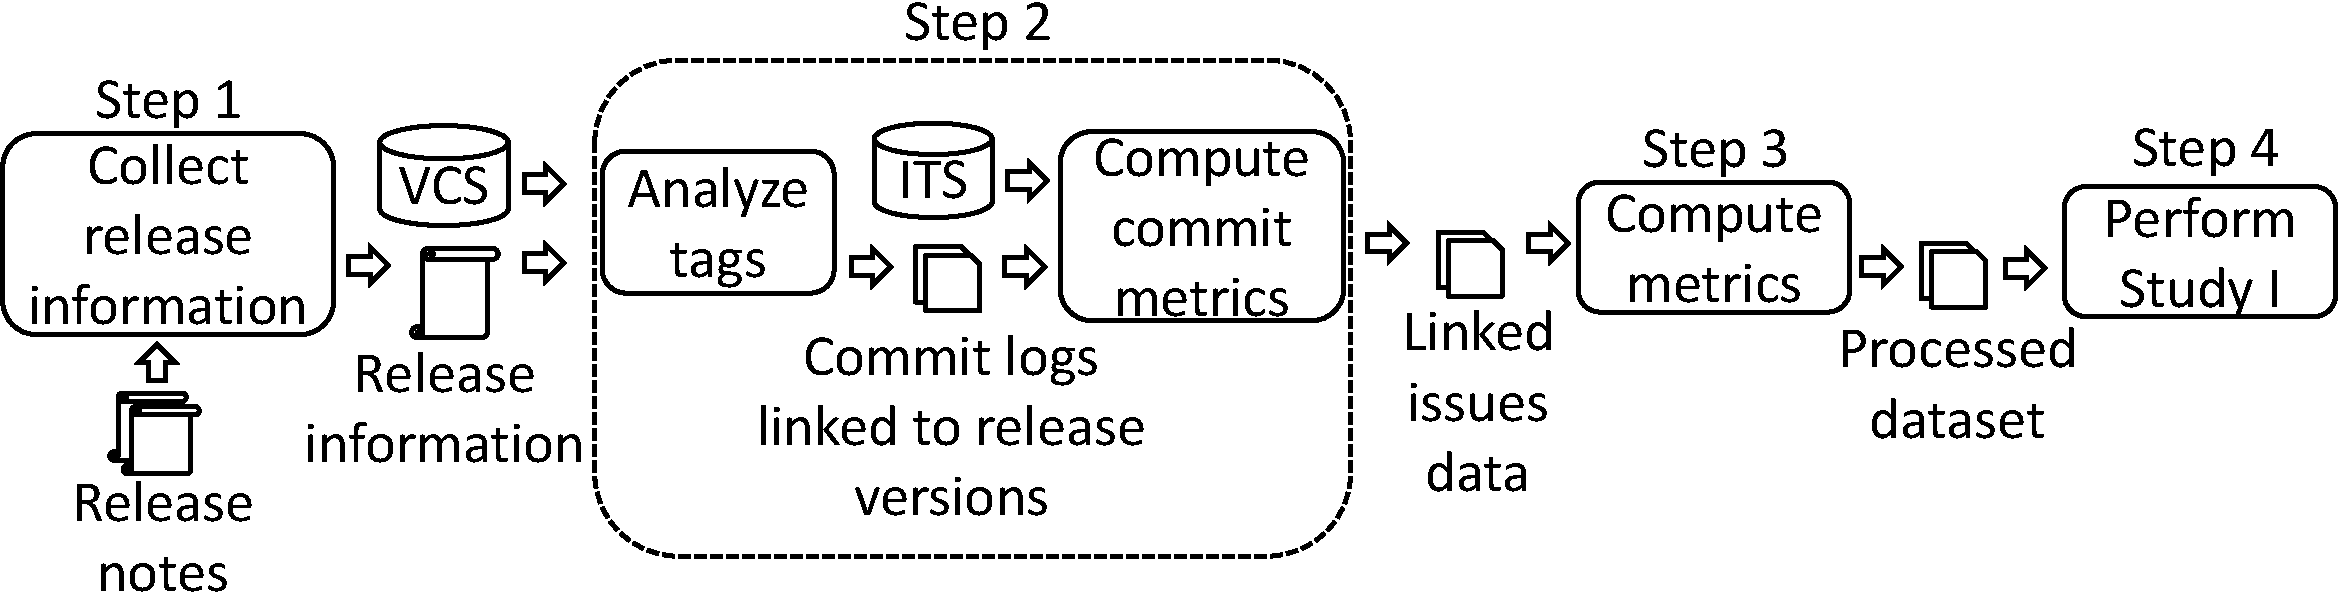
\includegraphics[width=0.90\textwidth,keepaspectratio]
	{chapters/chapter5/figures/database_construction_final.pdf}
	\caption{
		Overview of the process to construct the dataset that is used in
		our \hyperref[st:study3]{Study}~\ref{st:study3}.
	}
	\label{fig:database_construction}
\end{figure}

\begin{table}[!]
	\footnotesize
	\centering
	\caption{The studied traditional and rapid Firefox releases.
	\label{tbl:releases}}
		\begin{tabular}{ccccc}
			\hline 
			\textbf{Strategy} & \textbf{Version range} &
			\textbf{Time period} & \textbf{\# of Majors} &
			\textbf{\# of Minors}\tabularnewline
			\hline 
			\hline 
			Trad. & 1.0 - 4.0 & Sep/2004 - Mar/2012 & 7 & 104\tabularnewline
			\hline 
			Rapid & 5 - 27 & Jun/2011 - Sep/2014 & 23 & 50\tabularnewline
			\hline 
		\end{tabular}%
	%	}
\end{table}

\noindent\textbf{\textit{Step 1: Collect release information.}} We collect the date and
version number of each Firefox release (minor and major releases of each release
strategy) using the Firefox release history
wiki.\smartfoot{\url{https://en.wikipedia.org/wiki/Firefox_release_history}}
\hyperref[tbl:releases]{Table}~\ref{tbl:releases} shows: {\em (i)}the range of versions of releases that we
investigate, {\em (ii)} the investigated time period of each release strategy, and
(iii) the number of major and minor studied releases in each release strategy.\\

\noindent\textbf{\textit{Step 2: Link issues to releases.}} Once we collect the release
information, we use the \textit{tags} within the VCS to link issue IDs to
releases.  First, we analyze the tags that are recorded within the VCS. Since
Firefox migrated from CVS to Mercurial during release 3.5, we collect the tags
of releases 1.0 to 3.0 from CVS, while we collect the tags of releases 3.5 to 27
from
Mercurial.\smartfoot{\url{http://cvsbook.red-bean.com/cvsbook.html}}$^,$\smartfoot{\url{https://mercurial.selenic.com/}}
By analyzing the tags, we extract the commit logs within each tag. The extracted
commit logs are linked to their respective tags. We then parse the commit logs
to collect the issue IDs that are being addressed in the commits. We discard the
following patterns of potential issue IDs that are false positives:

\begin{enumerate}
\item Potential IDs that have less than five digits, since the issue IDs of the
	investigated releases should have at least five digits (2,559 issues
	were discarded).  
\item Commit logs that follow the pattern: ``Bug $<$ID$>$ -
	reftest'' or ``Bug $<$ID$>$ - JavaScript Tests'',
	which refer to tests and not bug fixes (269 issues were
	discarded).  
\item Any potential ID that is the name of a file, \eg
	``159334.js'' (607 issues were discarded).
\end{enumerate}          

We find that all of the remaining IDs match issue IDs that exist in the Firefox
ITS.

Since the commit logs are linked to VCS tags, we are also able to link the
issue IDs found within these commit logs to the releases that correspond to
those tags. For example, since we find the fix for issue 529404 in the commit
log of tag 3.7a1, we link this issue~ID to that release. We also merge together
the data of development releases like 3.7a1 into the nearest minor or major
release. For example, release 3.7a1 would be merged with release 4.0, since it
is the next user-intended release after 3.7a1. In the case that a particular
issue is found in the commit logs of multiple releases, we consider that
particular issue to pertain to the earliest release that contains the last fix
attempt (commit log), since that release is the first one to contain the
complete fix for the issue. Finally, we collect the issue report information
of each remaining issue (\eg opening date, fix date, severity, priority, and
description) using the ITS. Moreover, since the minor-rapid releases are
\textit{off-cycle releases}, in which addressed issues may skip being integrated
into \code{mozilla-central} (\ie NIGHTLY) tags, we manually collect the addressed
issues that were integrated into those releases using the Firefox release notes
(\ie 247 addressed~issues).\smartfoot{\url{https://www.mozilla.org/en-US/firefox/releases/}}
We add the manually collected addressed issues from ESR releases within the rapid
releases data, since they also represent data from a rapid release strategy.\\

\noindent\textbf{\textit{Steps 3 and 4: Compute metrics and perform analyses.}}
We use the data from Step 2 to compute the metrics that we use in our analyses.
We select these metrics (which are described in the
\hyperref[ch5:rq3]{approach for RQ3}) because we suspect that they
share a relationship with delivery delay.

\section{Results} \label{ch4:results}

In this study, we address three research
questions about the shift from a traditional to a rapid release cycle. The
motivation of each research question is detailed below.

\subsection{RQ1: Are addressed issues delivered more quickly in rapid
releases?}\label{ch5:rq1} 

\subsubsection*{RQ1: Motivation} 

Since there is a lack of empirical evidence to indicate that rapid release
cycles deliver addressed issues more quickly than traditional release cycles, we
compare the delivery delay of addressed issues in traditional releases against
the delivery delay in rapid releases in \hyperref[ch5:rq1]{RQ1}.\\

\subsubsection*{RQ1: Approach}

\begin{figure}[t!]
	\centering
	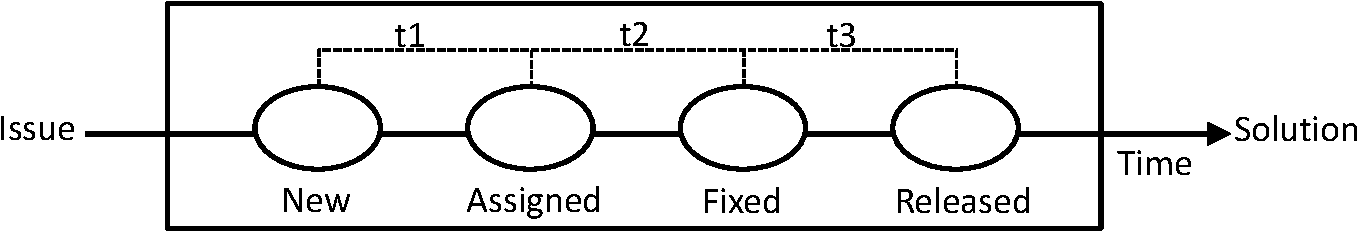
\includegraphics[width=\columnwidth,keepaspectratio]
	{chapters/chapter5/figures/rq1/issue_lifecycle.pdf}
	\caption{A simplified life cycle of an issue.}
	\label{fig:issue_lifecycle}
\end{figure}

\hyperref[fig:issue_lifecycle]{Figure}~\ref{fig:issue_lifecycle} shows a
simplified life cycle of an issue, which includes the triaging phase ({\em t1}),
the fixing phase ({\em t2}), and the integration phase ({\em t3}). We consider
the last RESOLVED-FIXED status as the moment at which a particular issue was
addressed (the fixed state in
\hyperref[fig:issue_lifecycle]{Figure}~\ref{fig:issue_lifecycle}). The
\textit{lifetime} of an issue is composed of all three phases (from \textit{new}
to \textit{released}). For \hyperref[ch5:rq1]{RQ1}, we first observe the lifetime of the issues of
traditional and rapid releases.  Next, we look at the time span of the
\textit{triaging}, \textit{fixing}, and \textit{integration} phases within the
lifetime of an issue.

We use beanplots~\cite{kampstra2008beanplot} to compare the distributions of our
data. The vertical curves of beanplots summarize and compare the distributions
of different datasets (see
\hyperref[fig:delivery_delay]{Figure}~\ref{fig:delivery_delay}). The higher
the frequency of data within a particular value, the thicker the bean is plotted
at that particular value on the $y$ axis. We also use Mann-Whitney-Wilcoxon
(MWW) tests~\cite{wilks2011statistical} and Cliff's delta effect-size
measures~\cite{cliff1993dominance}. MWW tests are non-parametric tests of the
\textit{null hypothesis} that two distributions come from the same population
($\alpha=0.05$). On the other hand, Cliff's delta is a non-parametric
effect-size measure to verify the difference in magnitude of one distribution compared
to another distribution. The higher the value of the Cliff's delta,
the greater the difference of values between distributions. For instance, if we
obtain a significant $p$ value but a small Cliff's delta, this means that
although two distributions do not come from the same population their 
difference is not that large. A positive Cliff's delta indicates how much
larger the values of the first distribution are, while a negative Cliff's delta
indicates the inverse. Finally, we use the \textit{Median Absolute Deviation}
(MAD) \cite{howell2005median,leys2013detecting} as a measure of the variation of
our distributions. The MAD is the median of the \textit{absolute deviations}
from one distribution's median. The higher the MAD, the greater is the variation
of a distribution with respect to its median.

\subsubsection*{RQ1: Results}

\begin{figure}[t!]
	\centering
	\subfloat[Lifetime]{
		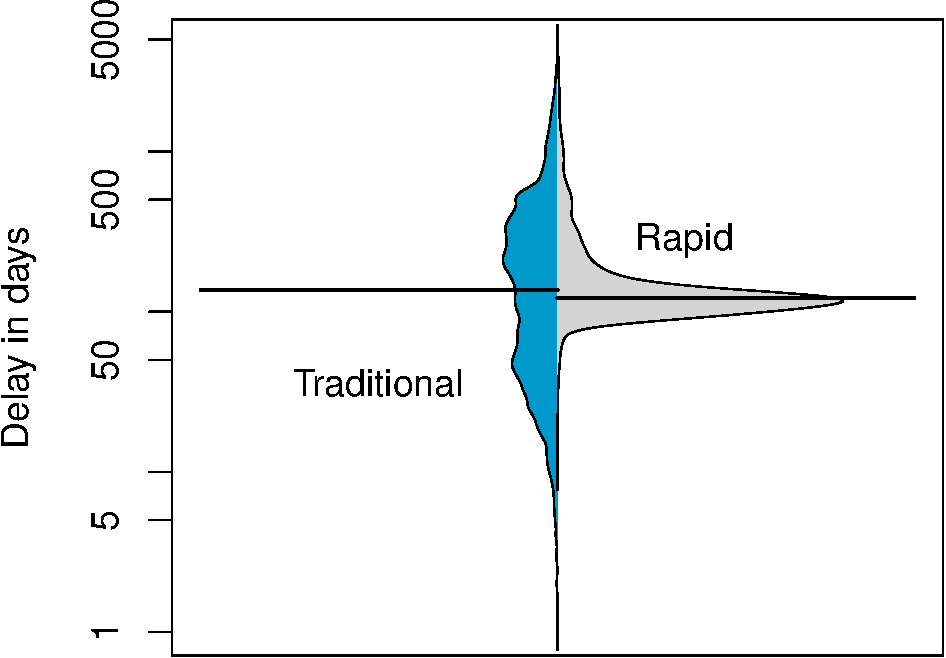
\includegraphics[width=.45\columnwidth,keepaspectratio]
		{chapters/chapter5/figures/rq1/trad-vs-rapid-entire.pdf}
		\label{fig:delivery_delay}
	}
	\subfloat[Triaging phase]{
		\centering
		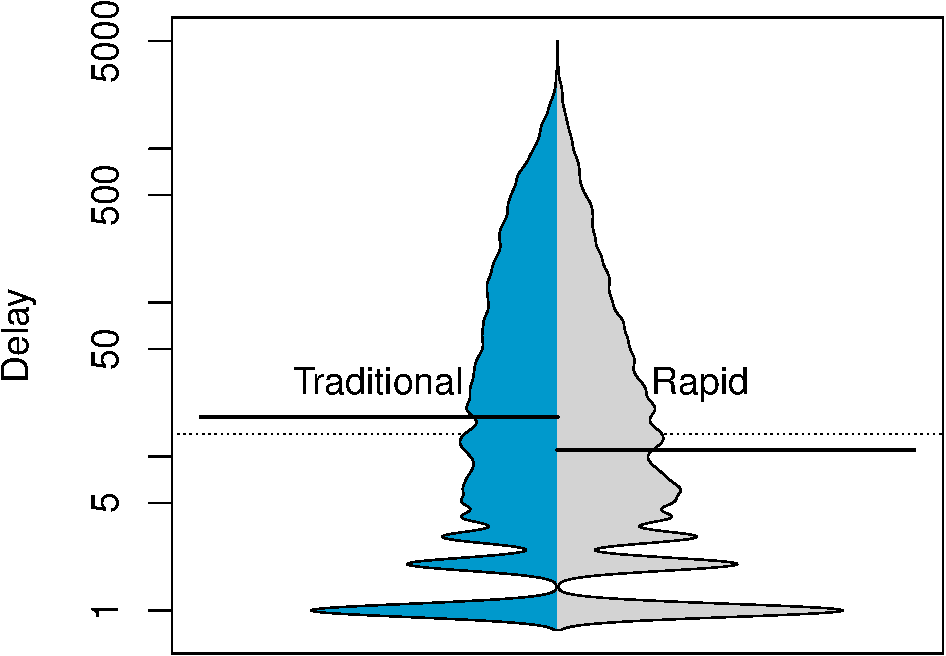
\includegraphics[width=.45\columnwidth,keepaspectratio]
		{chapters/chapter5/figures/rq1/traditional_vs_rapid_triaging.pdf}
		\label{fig:triaging}
	}

	\subfloat[Fixing phase]{
		\centering
		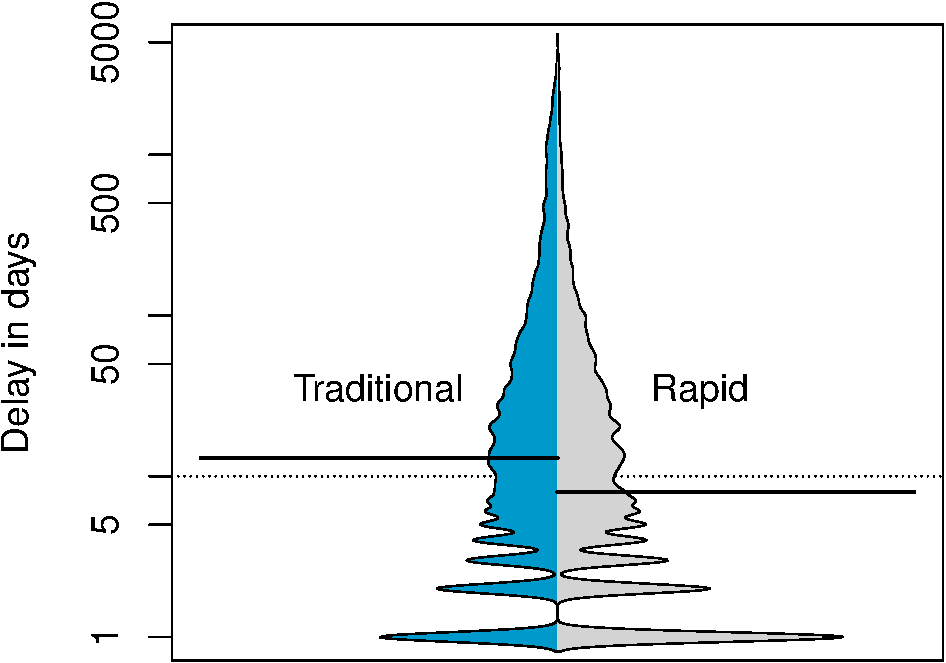
\includegraphics[width=.45\columnwidth,keepaspectratio]
		{chapters/chapter5/figures/rq1/traditional_vs_rapid_fixtime.pdf}
		\label{fig:fixtime}
	}
	\subfloat[Integration phase]{
		\centering
		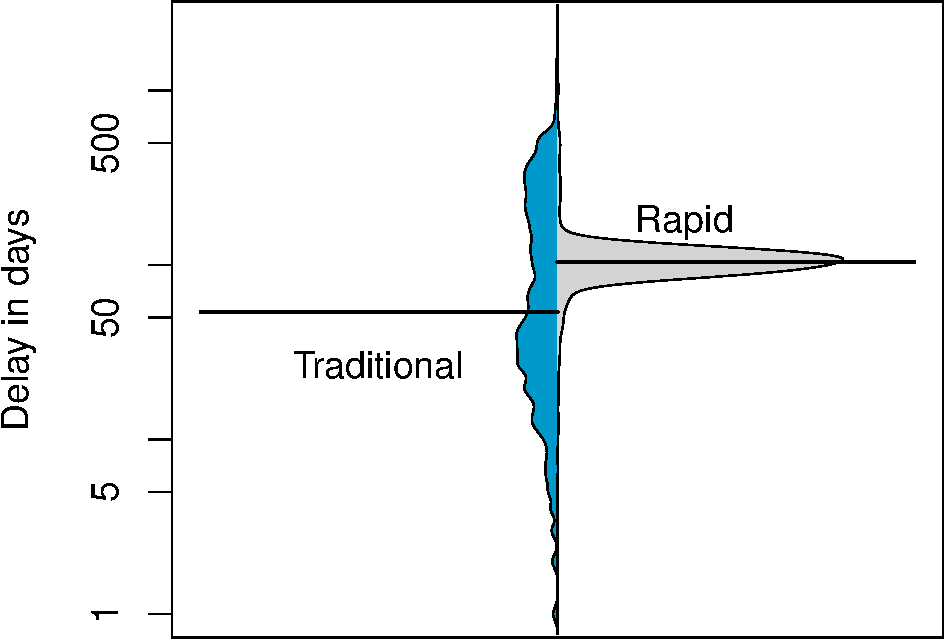
\includegraphics[width=.45\columnwidth,keepaspectratio]
		{chapters/chapter5/figures/rq1/traditional_vs_rapid.pdf}
		\label{fig:traditional_vs_rapid}
	}
	\caption{Time spans of the phases involved in the lifetime of an issue.}
	\label{fig:timespans}
\end{figure}

\noindent\textit{\textbf{Observation~1---There is no significant difference between traditional
and rapid releases regarding issue lifetime.}}\observation{obs:1}
\hyperref[fig:delivery_delay]{Figure}~\ref{fig:delivery_delay} shows the distributions of the lifetime of the
issues in traditional and rapid releases. We observe a $p<1.03e^{-14}$ but a
$negligible$ difference between the distributions ($\textit{delta}=0.03$). We
also observe that traditional releases have a greater MAD ($154$ days) than
rapid releases ($29$ days), which indicates that rapid releases are more
consistent with respect to the lifetime of the issues. Our results indicate that
the difference in the issues' lifetime between traditional and rapid releases is
not as obvious as one might expect. We then look at the triaging, fixing, and
integration time spans to better understand the differences between traditional
and rapid releases.\\

\noindent\textit{\textbf{Observation~2---Addressed issues are triaged and fixed more quickly in
rapid releases, but tend to wait for a longer time before being
delivered.}}\observation{obs:2}
\hyperref[fig:triaging]{Figures}~\ref{fig:triaging}~,~\ref{fig:fixtime},~and~\ref{fig:traditional_vs_rapid}
show the triaging, fixing, and integration time spans, respectively. We observe
that addressed issues take a median time of 54 days to be integrated into
traditional releases, while taking 104 days (median) to be integrated into rapid
releases. We observe a $p<2.2e^{-16}$ with a $small$ effect-size
($delta=-0.25$).

Regarding fixing time span, an issue takes 6 days (median) to be fixed in
rapid releases, and 9 days (median) in traditional releases. These results
are statistically significant $p<2.2e^{-16}$, but there is only a $negligible$
difference between distributions ($delta=0.13$). 

Our results complement previous research. Khomh~\etal \cite{khomh2012faster}
found that post- and pre-release bugs that are associated with crash reports are
fixed faster in rapid Firefox releases than in traditional releases.
Furthermore, we observe a significant $p<2.2e^{-16}$ but $negligible$
difference ($\textit{delta}=0.11$) between traditional and rapid releases
regarding triaging time. The median triaging time for rapid and traditional
releases are 11 and 18 days, respectively.

When we consider both pre-integration phases together (triaging $t1$ plus
fixing $t2$ in \hyperref[fig:issue_lifecycle]{Figure}~\ref{fig:issue_lifecycle}), we observe that an issue takes
$11$ days (median) to triage and address in rapid releases, while
it takes $19$ days (median) in traditional releases. We observe a $p<2.2e^{-16}$ with a $small$
effect-size ($delta=0.15$). Our results suggest that even though issues have
shorter pre-integration phases in rapid releases, they remain ``on the
shelf'' for a longer time on average.

Finally, we again observe that rapid releases are more consistent than
traditional releases in terms of fixing and integration rate. Rapid releases
achieve MADs of 9 and 17 days for fixing and integration, respectively. The
values for traditional releases are 13 and 64 days for fixing and integration,
respectively.\\ 

\conclusionbox{Although issues are triaged and fixed faster in rapid releases,
they tend to take a longer time to be integrated. However, the delivery rate
of addressed issues is more consistent in rapid releases than in traditional
ones.}

\subsection{RQ2: Why can traditional releases deliver addressed issues
more quickly?}\label{ch5:rq2} 

\subsubsection*{RQ2: Motivation} 

In \hyperref[ch5:rq1]{RQ1}, we surprisingly find that traditional releases tend
to deliver addressed issues more quickly than rapid releases. This result raises
the following question: why can a traditional release strategy, which has a
longer release cycle, deliver addressed issues more quickly than a rapid
release~strategy?\\

\subsubsection*{RQ2: Approach}

In \hyperref[ch5:rq2]{RQ2}, we group traditional and rapid releases into major
and minor releases and study their delivery delays. As in
\hyperref[ch5:rq1]{RQ1}, we also use beanplots~\cite{kampstra2008beanplot}, MWW
tests~\cite{wilks2011statistical}, and Cliff's delta effect-size
measures~\cite{cliff1993dominance} to perform our comparisons.

\subsubsection*{RQ2: Results}

\begin{figure}[t!]
	\centering
	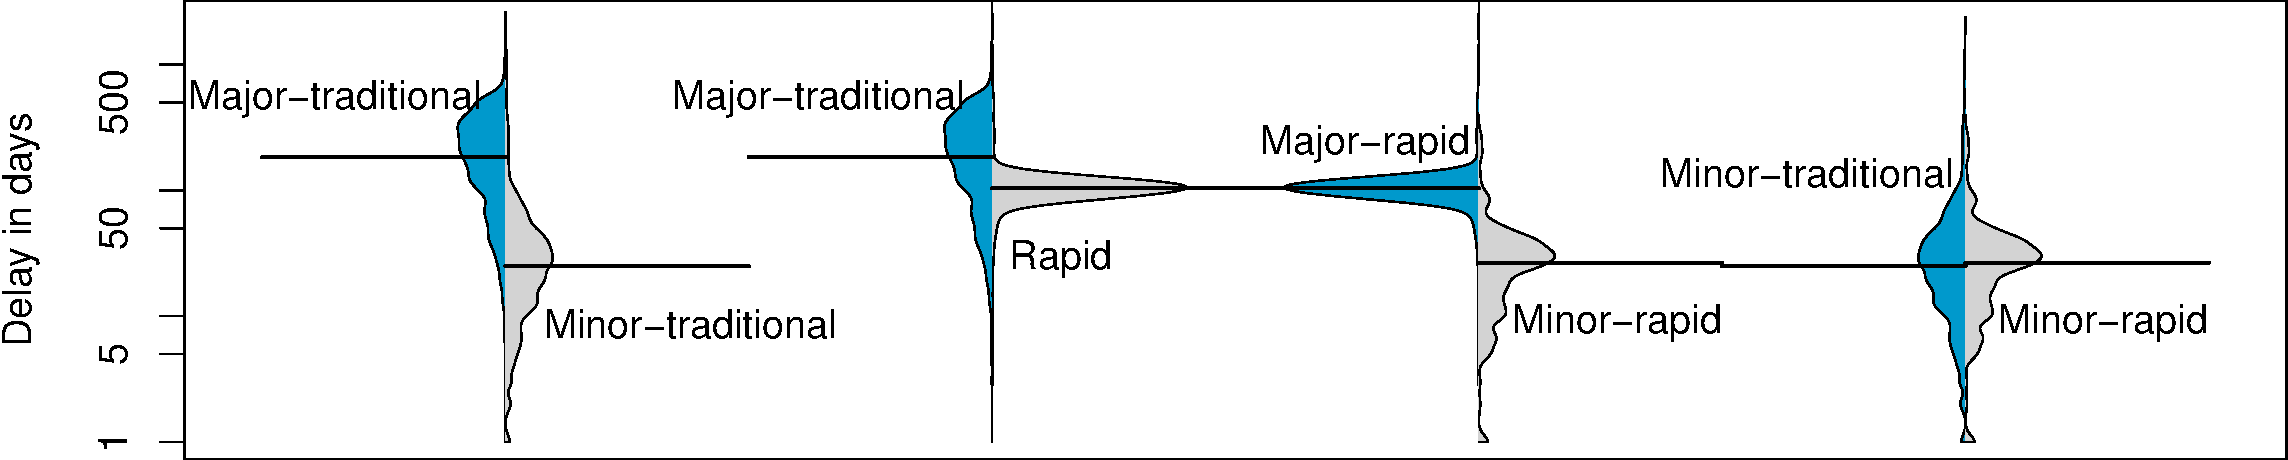
\includegraphics[width=\textwidth,keepaspectratio]
	{chapters/chapter5/figures/rq2/major_vs_minor.pdf}
	\caption{
		Distributions of delivery delay of addressed issues grouped by minor and major
		releases.
	}
	\label{fig:major_vs_minor}
\end{figure}

\begin{sloppypar}
\noindent\textit{\textbf{Observation~3---Minor-traditional releases tend to have
less delivery delay than major/minor-rapid releases.}}\observation{obs:3}
\hyperref[fig:major_vs_minor]{Figure}~\ref{fig:major_vs_minor} shows the distributions of delivery delay
grouped by (1) \textit{major-traditional vs. minor-traditional}, (2)
\textit{major-traditional vs. rapid}, (3) \textit{major-rapid vs. minor-rapid},
and (4) \textit{minor-traditional vs. minor-rapid}. In the comparison of
\textit{major-traditional vs.  minor-traditional}, we observe that
minor-traditional releases are mainly associated with shorter delivery delay.
Furthermore, in the comparison \textit{major-traditional vs. rapid}, rapid
releases deliver addressed issues more quickly than major-traditional releases
on average ($p<2.2e^{-16}$ with a $medium$ effect-size, \ie  $delta=0.40$). 
\end{sloppypar}

The Firefox rapid release cycle includes ESR releases (see
\hyperref[ch:background]{Chapter}~\ref{ch:background}) and a few minor
stabilization and security releases. These releases also deliver addressed
issues more quickly than major-rapid releases (\textit{major-rapid vs.
minor-rapid}) with a $p<2.2e^{-16}$ and a $large$ effect-size, \ie $delta=0.92$.
Furthermore, we do not observe a statistically significant difference between
distributions in the comparison of \textit{minor-traditional vs. minor-rapid}
($p=0.68$).

Minor-traditional releases have the lowest delivery delay (median of 25
days). This is likely because they are more focused on a particular set of
issues that, once addressed, should be released immediately. For example, the
release history documentation of Firefox shows that minor releases are usually
related to stability and security
issues.\footnote{\url{https://www.mozilla.org/en-US/firefox/releases/}}\\

\begin{figure}[t!]
	\centering
	\subfloat[Only Major]{           
		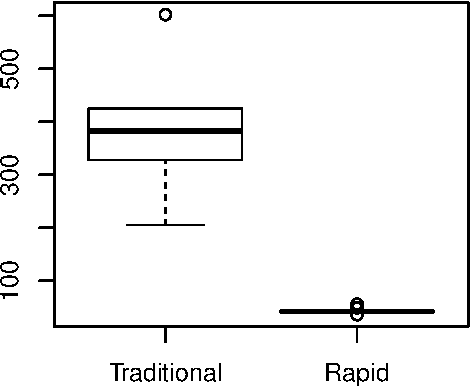
\includegraphics[width=0.45\columnwidth,keepaspectratio]
		{chapters/chapter5/figures/releases/majorreleases_length.pdf}
		\label{fig:majorreleases_length}
	}
	\subfloat[Major and Minor]{
		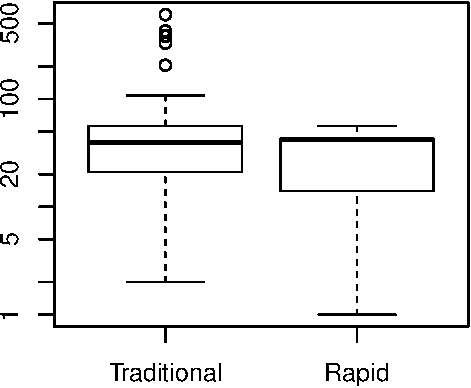
\includegraphics[width=0.45\columnwidth,keepaspectratio]
		{chapters/chapter5/figures/releases/releases_length.pdf}
		\label{fig:releases_length}
	}
	\caption{Release frequency (in days). The outliers in figure~(b)
		represent the major-traditional releases.}
	\label{fig:release_length_analysis}
\end{figure}

\noindent\textit{\textbf{Observation~4---When considering both
minor and major releases, the time span between traditional and rapid releases
are roughly the same.}}\observation{obs:4}
Since we observe that delivery delay is shorter on average in traditional
releases, we also investigate the length of the release cycles to better
understand our previous results (see \hyperref[obs:2]{Observation}~\ref{obs:2}).
\hyperref[fig:majorreleases_length]{Figure}~\ref{fig:majorreleases_length} shows that, at first glance, one may
speculate that rapid releases should deliver addressed issues more quickly
because releases are produced more frequently.  However, if we consider both
major and minor releases---as shown in \hyperref[fig:releases_length]{Figure}~\ref{fig:releases_length}---we
observe that both release strategies deliver releases at roughly the same rate
on average (median of $40$ and $42$ days for traditional and rapid releases,
respectively).\\

\conclusionbox{
Minor-traditional releases are one of the main reasons why the traditional
release strategy can deliver addressed issues more quickly than the rapid
release strategy. Furthermore, the lengths of the release cycles are roughly the
same between traditional and rapid releases when both minor and major releases
are considered.
}

\subsection{RQ3: Did the change in the release strategy have an impact on
the characteristics of delayed issues?}\label{ch5:rq3} 

\subsubsection*{RQ3: Motivation}

In \hyperref[ch5:rq1]{RQ1} and \hyperref[ch5:rq2]{RQ2}, we study the differences
between rapid and traditional releases with respect to delivery delay. We find
that although issues tend to be addressed more quickly in rapid releases, they
tend to wait longer to be delivered. We also find that the use of minor releases
is a key reason as to why traditional releases may deliver addressed issues more
quickly. In \hyperref[ch4:rq3]{RQ3}, we investigate what are the characteristics
of each release strategy that are associated with delivery delays. This
important investigation sheds light on what may generate delivery delays in each
release strategy, so that projects are aware of the characteristics of rapid
releases versus traditional releases before choosing to adopt one of these
release strategies. 

\subsubsection*{RQ3: Approach}

\begin{table}[!t]
	\footnotesize
	\caption{Metrics that are used in our explanatory models (Reporter, Resolver,
		and Issue families).
	\label{tbl:factors1}}
	\centering
		\begin{tabular}{rp{2cm}lp{9cm}}
			\hline
			\multicolumn{1}{c}{\textbf{Family}} &
			\multicolumn{1}{c}{\textbf{Metrics}} & \multicolumn{1}{c}{\textbf{Value}} &
			\multicolumn{1}{c}{\textbf{Definition (d)$\vert$Rationale (r)}}
			\\ \hline
			\multicolumn{ 1}{r}{\textbf{Reporter}} & Experience & Numeric & 
			\begin{tabular}{p{8.7cm}}
				\textbf{d:} the number of previously delivered issues that were reported by
				the reporter of a particular addressed issue.  \\ \hline 
				\textbf{r:} The greater the experience of the reporter the
				higher the quality of his/her reports and the
				solution to his/her reports might be delivered
				more quickly~\cite{shihab2010predicting}.
			\end{tabular}
			\\ \cline{2- 4}
			\multicolumn{ 1}{r}{} & Reporter integration & Numeric &
			\begin{tabular}{p{8.7cm}}
				\textbf{d:} The median in days of the previously delivered addressed issues
				that were reported by a particular reporter.
				\\ \hline 
				\textbf{r:} If a particular reporter usually reports issues that are
				delivered quickly, his/her future reported issues might be delivered
				quickly as well.
			\end{tabular}
			\\ \hline
			\multicolumn{ 1}{r}{\textbf{Resolver}} & Experience & Numeric & 
			\begin{tabular}{p{8.7cm}}
				\textbf{d:} the number of previously delivered addressed issues that were
				addressed by the resolver of a particular
				addressed issue. We consider the collaborator
				that changed the status of an issue to
				RESOLVED-FIXED as the resolver of that issue. \\ \hline 
				\textbf{r:} The greater the experience of the resolver, the
				greater the likelihood that his/her code will be
				delivered faster~\cite{shihab2010predicting}.
			\end{tabular}
			\\ \cline{2- 4}
			\multicolumn{ 1}{r}{} & Resolver integration & Numeric &
			\begin{tabular}{p{8.7cm}}
				\textbf{d:} The median in days of the previously delivered addressed issues
				that were addressed by a particular resolver.
				\\ \hline 
				\textbf{r:} If a particular resolver usually address issues that are
				delivered quickly, his/her future addressed issues might be delivered
				quickly as well.
			\end{tabular}
			\\ \hline
			\multicolumn{ 1}{r}{\textbf{Issue}} & Stack trace attached & Boolean &
			\begin{tabular}{p{8.7cm}}
				\textbf{d:} We verify if the issue report has a stack trace attached in its description. \\ \hline 
				\textbf{r:} A stack trace attached may provide useful information regarding
				the cause of the issue, which may quicken the integration of
				the addressed issue~\cite{schroter2010stack}. 
			\end{tabular}
			\\ \cline{2- 4}
			\multicolumn{ 1}{r}{} & Severity & Nominal &
			\begin{tabular}{p{8.7cm}}
				\textbf{d:} The severity level of the issue report. Issues with higher
				severity levels (\eg blocking) might be delivered faster than other issues.
				\\ \hline 
				\textbf{r:} Panjer observed that the severity of an issue has a large effect
				on its time to be addressed in the Eclipse project~\cite{Panjer2007}.
			\end{tabular}
			\\ \cline{2- 4}
			\multicolumn{ 1}{r}{} & Priority & Nominal &
			\begin{tabular}{p{8.7cm}}
				\textbf{d:} The priority level of the issue report. Issues with higher
				priority levels (\eg P1) might be delivered faster than other issues.
				\\ \hline 
				\textbf{r:} Higher priority issues will likely be delivered before lower
				priority issues.
			\end{tabular}
			\\ \cline{2- 4}
			\multicolumn{ 1}{r}{} & Description size & Numeric &
			\begin{tabular}{p{5.6cm}}
				\textbf{d:} The number of words in the description of the issue. 
				\\ \hline 
				\textbf{r:} Issues that are well described might be more easy to integrate
				than issues that are difficult to understand.
			\end{tabular}
			\\ \hline
		\end{tabular}
\end{table}

\begin{table}[!t]
	\footnotesize
	\caption{Metrics that are used in our explanatory models (Project family).
	\label{tbl:factors2}}
	\centering
		\begin{tabular}{rp{2cm}lp{9cm}}
			\hline
			\multicolumn{1}{c}{\textbf{Family}} &
			\multicolumn{1}{c}{\textbf{Metrics}} & \multicolumn{1}{c}{\textbf{Value}} &
			\multicolumn{1}{c}{\textbf{Definition (d)$\vert$Rationale (r)}}
			\\ \hline
			\multicolumn{ 1}{r}{\textbf{Project}} & Queue rank & Numeric &
			\begin{tabular}{p{8.7cm}}
				\textbf{d:} A rank number that represents the
				moment at which an issue is
				addressed compared to other addressed issues in the backlog. For instance,
				in a backlog that contains $500$ issues, the first addressed issue has
				a rank of~1, while the last addressed issue has
				a rank of 500.
				\\ \hline 
				\textbf{r:} An issue with a high \textit{queue rank} is a recently
				addressed issue. An addressed issue might be delivered faster/slower
				depending of its rank.
			\end{tabular}
			\\ \cline{2- 4}
			\multicolumn{ 1}{r}{} & Cycle queue rank & Numeric &
			\begin{tabular}{p{8.7cm}}
				\textbf{d:} A rank number that represents the
				moment at which an issue is
				addressed compared to other addressed issues of the same release cycle. For
				example, in a release cycle that contains $300$ addressed issues, the first
				addressed issue has a rank of $1$, while the
				last one has a rank of $300$.
				\\ \hline 
				\textbf{r:} An issue with a high \textit{cycle queue rank} is a recently
				addressed issue compared to the others of the same release cycle. An issue
				addressed close to the upcoming release might be delivered faster.
			\end{tabular}
			\\ \cline{2- 4}
			\multicolumn{ 1}{r}{} & Queue position & Numeric &
			\begin{tabular}{p{8.7cm}}
				\textbf{d:} $\frac{\text{queue rank}}{\text{all addressed issues}}$. The
				\textit{queue rank} is divided by all the issues that are addressed by the
				end of the next release. A \textit{queue position} close to 1 indicates that the
				issue was addressed recently compared to others in the backlog.
				\\ \hline 
				\textbf{r:} An addressed issue
				might be delivered faster/slower depending of its position.
			\end{tabular}
			\\ \cline{2- 4}
			\multicolumn{ 1}{r}{} & Cycle queue position & Numeric &
			\begin{tabular}{p{8.7cm}}
				\textbf{d:} $\frac{\text{cycle queue rank}}{\text{addressed issues of the
				current cycle}}$. The \textit{cycle queue rank} is divided by all of the
				addressed issues of the release cycle. A \textit{cycle
				queue position} close to 1 indicates that the issue was addressed recently
				in the release cycle.
				\\ \hline 
				\textbf{r:}  An issue addressed close
				to a upcoming release might be delivered faster. 
			\end{tabular}
			\\ \hline
		\end{tabular}
\end{table}

\begin{table}[!t]
	\footnotesize
	\caption{Metrics that are used in our explanatory models (Process family).
	\label{tbl:factors3}}
	\centering
		\begin{tabular}{rp{2cm}lp{9cm}}
			\hline
			\multicolumn{1}{c}{\textbf{Family}} &
			\multicolumn{1}{c}{\textbf{Metrics}} & \multicolumn{1}{c}{\textbf{Value}} &
			\multicolumn{1}{c}{\textbf{Definition (d)$\vert$Rationale (r)}}
			\\ \hline
			\multicolumn{ 1}{r}{\textbf{Process}} & Number of Impacted Files & Numeric & 
			\begin{tabular}{p{8.7cm}}
				\textbf{d:} The number of files that are linked to an issue report. \\ \hline 
				\textbf{r:} A delivery delay might be
				related to a high number of impacted files 
				because more effort would be required to properly integrate the modifications 
				\cite{Jiang2013}. 
			\end{tabular}
			\\ \cline{ 2- 4}
			\multicolumn{ 1}{r}{} & Churn & Numeric &
			\begin{tabular}{p{8.7cm}}
				\textbf{d:} The sum of added lines plus the sum
				of deleted lines to address the issue.\\ \hline 
				\textbf{r:} A higher churn suggests that a great amount of work was required
				to address the issue, and hence, verifying the impact of integrating the
				modifications may also be difficult~\cite{Jiang2013,Nagappan2005}.
			\end{tabular}
			\\ \cline{2- 4}
			\multicolumn{ 1}{r}{} & Fix time & Numeric &
			\begin{tabular}{p{8.7cm}}
				\textbf{d:} Number of days between the date when
				the issue was
				triaged and the
				date that it was addressed~\cite{Giger2010}. \\ \hline 
				\textbf{r:} If an issue is addressed quickly, it may have a better chance to
				be delivered faster.
			\end{tabular}
			\\ \cline{ 2- 4}
			\multicolumn{ 1}{r}{} & Number of activities & Numeric &
			\begin{tabular}{p{8.7cm}}
				\textbf{d:} An activity is an entry in the issue's history. \\ \hline 
				\textbf{r:} A high number of activities might indicate that much work was
				required to address the issue, which may impact the integration of the
				issue into a release~\cite{Jiang2013}.
			\end{tabular}
			\\ \cline{ 2- 4}
			\multicolumn{ 1}{r}{} & Number of comments & Numeric & 
			\begin{tabular}{p{8.7cm}}
				\textbf{d:} The number of comments of an issue report. \\ \hline 
				\textbf{r:} A large number of comments might indicate the importance of an
				issue or the difficulty to understand it~\cite{Giger2010}, which might
				impact the delivery delay~\cite{Jiang2013}.
			\end{tabular}
			\\ \cline{ 2- 4}
			\multicolumn{ 1}{r}{} & Interval of comments & Numeric &
			\begin{tabular}{p{8.7cm}}
				\textbf{d:} The sum of the time intervals (hour) between
				comments divided by the total number of comments of an issue report. \\ \hline 
				\textbf{r:} A short \textit{interval of comments} indicates that an intense
				discussion took place, which suggests that the issue is important. Hence,
				such an issue may be delivered faster.   
			\end{tabular}
			\\ \cline{ 2- 4}
			\multicolumn{ 1}{r}{} & Number of tosses & Numeric &
			\begin{tabular}{p{8.7cm}}
				\textbf{d:} The number of times that the assignee has changed. \\ \hline 
				\textbf{r:} Changes in the issue assignee might indicate that more than one
				developer have worked on the issue. Such issues may be more difficult to
				integrate, since different expertise from different developers might 
				be required~\cite{Jeong2009,Jiang2013}.  
			\end{tabular}
			\\ \hline
		\end{tabular}
\end{table}

For \hyperref[ch5:rq3]{RQ3}, we build explanatory models (\ie logistic
regression models) for the traditional and rapid releases data using the metrics
that are presented in
\hyperref[tbl:factors1]{Tables}~\ref{tbl:factors1},~\ref{tbl:factors2}, and
\ref{tbl:factors3}. We model our response variable $Y$ as $Y=1$ for addressed
issues that are delayed, \ie had their delivery prevented in at least one
release\cite{costa2014empirical} and $Y=0$ otherwise. Hence, our models are
intended to explain why a given addressed issue has a delayed delivery (\ie
$Y=1$).

\begin{figure}[t!]
	\centering
	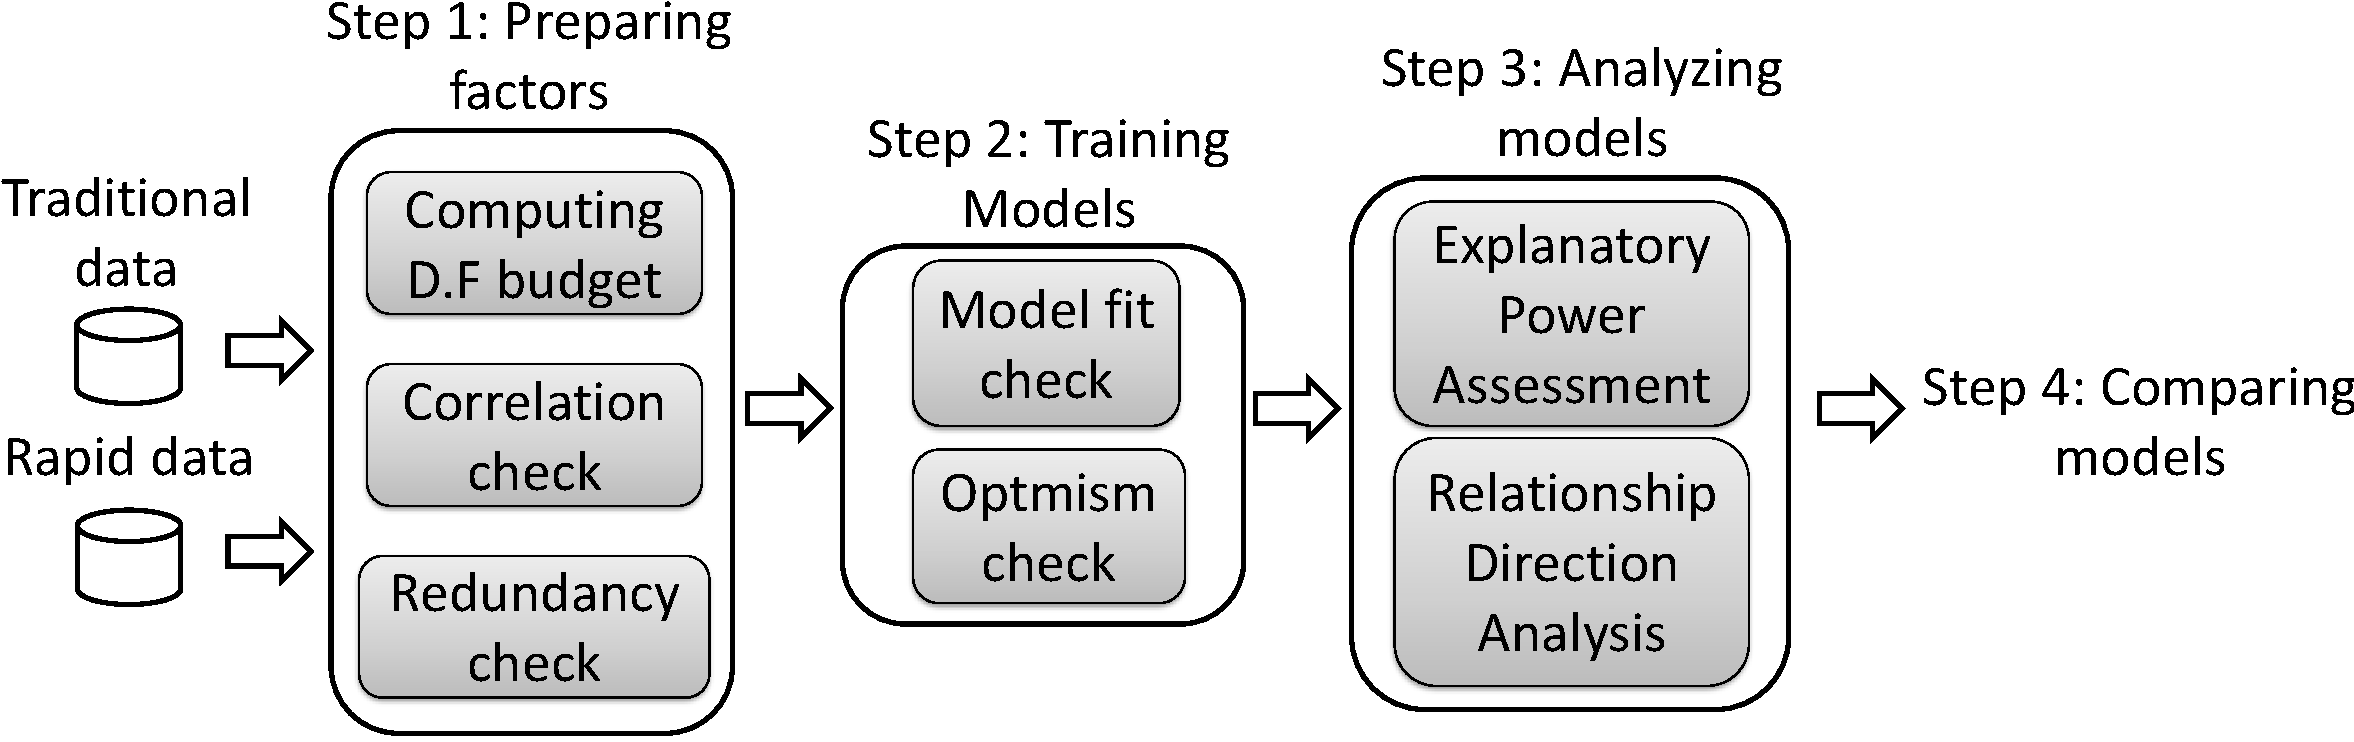
\includegraphics[width=\columnwidth,keepaspectratio]
	{chapters/chapter5/figures/rq3/model_construction.pdf}
	\caption{Overview of the process that we use to build our explanatory models.}
	\label{fig:model_construction}
\end{figure}

We follow the guidelines of Harrell~Jr.~\cite{harrell2001regression} for
building explanatory regression models.
\hyperref[fig:model_construction]{Figure}~\ref{fig:model_construction} provides
an overview of the process that we use to build our models. First, we estimate
the budget of degrees of freedom that we can spend on our models while having a
low risk of overfitting (\ie producing a model that is too specific to the
training data to be useful when applied to other unseen data). Second, we check for
metrics that are highly correlated using Spearman rank correlation tests
$(\rho)$ and we perform a redundancy analysis to remove any redundant metrics
before building our explanatory models. 

We then assess the fit of our models using the ROC area and the Brier score. The
ROC area is used to evaluate the degree of discrimination that is achieved by
a model. The ROC values range between 0 (worst) and 1 (best). An area greater
than 0.5 indicates that the explanatory model outperforms na\"{i}ve random
guessing models. The Brier score is used to evaluate the accuracy of
probabilistic predictions. This score measures the mean squared difference
between the probability of delay assigned by our models for a particular issue
$I$ and the actual outcome of $I$ (\ie whether $I$ is actually delayed or not).
Hence, the lower the Brier score, the more accurate the probabilities that are
produced by a model.

Next, we assess the stability of our models by computing the
\textit{optimism-reduced} ROC area and Brier score~\cite{efron1986biased}. The
optimism of each metric is computed by selecting a bootstrap sample to
fit a model with the same degrees of freedom of the original model. The model
that is trained using the bootstrap sample is applied both on the bootstrap and original
samples (ROC and Brier scores are computed for each sample). The optimism is the
difference in the ROC area and Brier score of the bootstrap sample and original
sample. This process is repeated 1,000 times and the average optimism is
computed. Finally, we obtain the \textit{optimism-reduced} scores by subtracting
the average optimism from the initial ROC area and Brier score
estimates~\cite{efron1986biased}.

We evaluate the impact of each metric on the fitted models using
Wald $\chi^2$ maximum likelihood tests. The larger the $\chi^2$ value, the
larger the impact that a particular metric has on our explanatory models'
performance. We also study the relationship that our metrics 
share with the likelihood of delivery delay. To do so, we plot the change in
the estimated probability of delay against the change in a given metric
while holding the other metrics constant at their median values using the
\code{Predict} function of the \code{rms} package~\cite{harrell2001regression}. 

We also plot nomograms~\cite{iasonos2008build,harrell2001regression} to evaluate
the impact of the metrics in our models. Nomograms are user-friendly charts that
visually represent explanatory models. For instance,
\hyperref[fig:nomogram_trad]{Figure}~\ref{fig:nomogram_trad} shows the nomogram
of the model that we fit for the rapid release data. The higher the number of
points that are assigned to an explanatory metric on the $x$ axis (\eg 100
points are assigned to \textit{comments} in rapid releases), the larger the
effect of that metric in the explanatory model. We compare which metrics are
more important in both traditional and rapid releases in order to better
understand the differences between these release strategies.

\subsubsection*{RQ3: Results}

\begin{sloppypar}
\noindent\textit{\textbf{Observation~5---Our models achieve a Brier score of 0.05-0.16 and ROC
areas of 0.81-0.83.}}\observation{obs:5}
The models that we fit to traditional releases achieve a Brier score of 0.16 and
an ROC area of 0.83, while the models that we fit to the rapid release data
achieve a Brier score of 0.05 and an ROC area of 0.81. Our models outperform
na\"{i}ve approaches such as random guessing and ZeroR---our ZeroR models
achieve ROC areas of 0.5 and Brier scores of 0.06 and 0.45 for rapid and
traditional releases, respectively. Moreover, the bootstrap-calculated optimism
is less than 0.01 for both the ROC areas and Brier scores of our models. This
result shows that our regression models are stable enough to perform the
statistical inferences that follow.\\

\begin{table}[t]
	\scriptsize
	\begin{center}
		\caption{Overview of the regression model fits. The $\chi^2$ of
		each metric is shown as the proportion in relation to the total
	$\chi^2$ of the model.  \label{tbl:regression_models} }
		%\resizebox{\textwidth}{!}{
			\begin{tabular}{cccc}
			\cline{3-4} 
			\multicolumn{2}{c}{} & 
			Traditional releases &
			Rapid releases 
			\tabularnewline
			\hline 
			\multicolumn{2}{c}{\# of instances} & 
			$34,673$ &
			$37,441$  
			\tabularnewline
			\hline
			\multicolumn{2}{c}{Wald $\chi^2$} & 
			$4,964$ &
			$2,705$  
			\tabularnewline
			\hline 
			\multicolumn{2}{c}{Budgeted Degrees of Freedom} &
			$1033$ & 
			$149$ 
			\tabularnewline
			\hline
			\multicolumn{2}{c}{Degrees of Freedom Spent} &
			$26$ & 
			$25$ 
			\tabularnewline
			%\hline 
			%\hline 
			%&  &  &  
			%\tabularnewline
			\hline 
			\multirow{2}{*}{Reporter experience} & 
			D.F. & 
			$1$ & 
			$1$  
			\tabularnewline 
			& 
			$\chi^2$ & 
			$2^{\ast\ast\ast}$ &  
			$2^{\ast\ast\ast}$ 
			\tabularnewline
			\hline 
			\multirow{2}{*}{Reporter integration} & 
			D.F. & 
			$1$ & 
			$1$  
			\tabularnewline 
			& 
			$\chi^2$ & 
			$5^{\ast\ast\ast}$ &  
			$4^{\ast\ast\ast}$ 
			\tabularnewline
			\hline 
			\multirow{2}{*}{Resolver Experience} & 
			D.F. & 
			$1$ & 
			\multirow{2}{*}{$\oslash$}
			\tabularnewline &
			$\chi^2$ & 
			$1^{\ast\ast\ast}$ &
			\tabularnewline 
			\hline 
			\multirow{2}{*}{Resolver integration} & 
			D.F. & 
			$1$ & 
			$1$  
			\tabularnewline 
			& 
			$\chi^2$ & 
			$2^{\ast\ast\ast}$ &  
			$5^{\ast\ast\ast}$ 
			\tabularnewline
			\hline 
			\multirow{2}{*}{Fix time} & 
			D.F. & 
			1 &
			1  
			\tabularnewline & 
			$\chi^2$ &
			$2^{\ast\ast\ast}$ &
			$8^{\ast\ast\ast}$ 
			\tabularnewline \hline 
			\multirow{2}{*}{Severity} &
			D.F. & 
			$6$ & 
			$6$ 
			\tabularnewline & 
			$\chi^2$ & 
			$1^{\ast\ast\ast}$ &  
			$1^{\ast\ast\ast}$  
			\tabularnewline \hline 
			\multirow{2}{*}{Priority} & 
			D.F. & 
			$5$ & 
			$5$ 
			\tabularnewline & 
			$\chi^2$ & 
			$1^{\ast\ast\ast}$ &  
			$\approx 0$   
			\tabularnewline \hline 
			\multirow{2}{*}{Size of description} & 
			D.F. & 
			$1$ &
			$1$  
			\tabularnewline & 
			$\chi^2$ & 
			$\approx 0$ &
			$1^{\ast\ast\ast}$   
			\tabularnewline \hline 
			\multirow{2}{*}{Stack trace attached} & 
			D.F. & 
			$1$ &
			$1$  
			\tabularnewline & 
			$\chi^2$ & 
			$\approx 0$ &  
			$\approx 0$ 
			\tabularnewline \hline 
			\multirow{2}{*}{Number of files} & 
			D.F. & 
			$1$ & 
			$1$
			\tabularnewline & 
			$\chi^2$ & 
			$1^{\ast\ast\ast}$ &  
			$1^{\ast\ast\ast}$ 
			\tabularnewline \hline 
			\multirow{2}{*}{Number of comments} & 
			D.F. & 
			$1$ &
			$1$ 
			\tabularnewline & 
			$\chi^2$ & 
			$\approx 0^{\ast}$ &  
			$31^{\ast\ast\ast}$  
			\tabularnewline \hline 
			\multirow{2}{*}{Number of tossing} & 
			D.F. & 
			$1$ &
			$1$  
			\tabularnewline & 
			$\chi^2$ & 
			$\approx 0^{\ast\ast\ast}$ &  
			$\approx 0$   
			\tabularnewline \hline 
			\multirow{2}{*}{Number of activities} & 
			D.F. & 
			$1$ &
			$1$  
			\tabularnewline & 
			$\chi^2$ & 
			$1^{\ast\ast\ast}$ &  
			$3^{\ast\ast\ast}$  
			\tabularnewline \hline 
			\multirow{2}{*}{Interval of comments} & 
			D.F. & 
			\multirow{2}{*}{$\oslash$} &
			\multirow{2}{*}{$\oslash$}  
			\tabularnewline &
			$\chi^2$ &
			&
			\tabularnewline \hline 
			\multirow{2}{*}{Code churn} & 
			D.F. & 
			$1$ & 
			$1$  
			\tabularnewline &
			$\chi^2$ &
			$\approx 0$ &  
			$\approx 0$ 
			\tabularnewline \hline 
			\multirow{2}{*}{Queue position} & 
			D.F. & 
			$1$ &             
			$1$
			\tabularnewline & 
			$\chi^2$ & 
			$17^{\ast\ast\ast}$ & 
			$2^{\ast\ast\ast}$
			\tabularnewline \hline 
			\multirow{1}{*}{Queue rank} & 
			D.F. & 
			$1$ & 
			$1$ 
			\tabularnewline &
			$\chi^2$ & 
			$56^{\ast\ast\ast}$ & 
			$14^{\ast\ast\ast}$
			\tabularnewline \hline 
			\multirow{2}{*}{Cycle queue rank} & 
			D.F. & 
			$1$ &
			$1$ 
			\tabularnewline &
			$\chi^2$ & 
			$10^{\ast\ast\ast}$ &
			$28^{\ast\ast\ast}$ 
			\tabularnewline \hline 
			\multirow{2}{*}{Cycle queue position} & 
			D.F. & 
			\multirow{2}{*}{$\oplus$} &
			\multirow{2}{*}{$\oslash$}  
			\tabularnewline &
			$\chi^2$ & 
			&
			\tabularnewline \hline 
		\end{tabular}
%	}
	\captionsetup{justification=centering}
	\caption*{
		$\oslash$ discarded during correlation analysis \\
		$\oplus$ discarded during redundancy analysis \\
		$\ast$ $p < 0.05$;
		$\ast\ast$ $p < 0.01$;
		$\ast\ast\ast$ $p < 0.001$\\ 
	}
	\end{center}
\end{table}

\noindent\textit{\textbf{Observation~6---Traditional releases prioritize the
delivery of backlog issues, while rapid releases prioritize the delivery
of issues of the current release cycle.}}\observation{obs:6}
\hyperref[tbl:regression_models]{Table}~\ref{tbl:regression_models} shows the explanatory power ($\chi^2$) of each
metric that we use in our models.  The \textit{queue rank} metric is the most
important metric in the models that we fit to the traditional release data.
Queue rank measures the moment when an issue is addressed in the backlog of the
project (see \hyperref[tbl:factors2]{Table}~\ref{tbl:factors2}).
\hyperref[fig:rankposition]{Figure}~\ref{fig:rankposition} shows the relationship that queue rank shares with
delivery delay. Our models reveal that the addressed issues in traditional
releases have a higher likelihood of being delayed if they are addressed later
when compared to other issues in the backlog of the project.   

\begin{figure}[t]
	\centering
	\subfloat{
		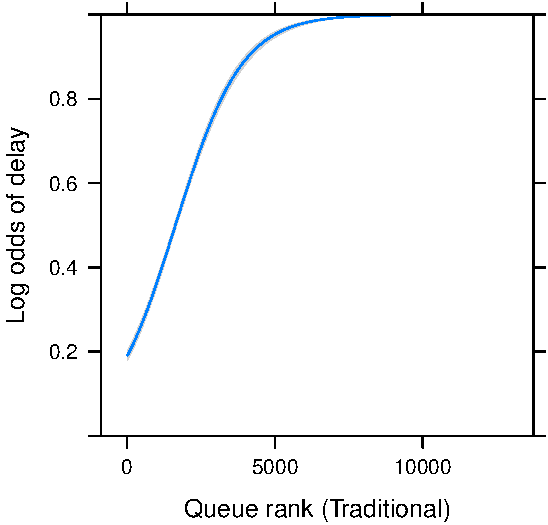
\includegraphics[width=0.43\textwidth,keepaspectratio]
		{chapters/chapter5/figures/rq3/queue_rank.pdf}
		\label{fig:rankposition}
	}
	\subfloat{
		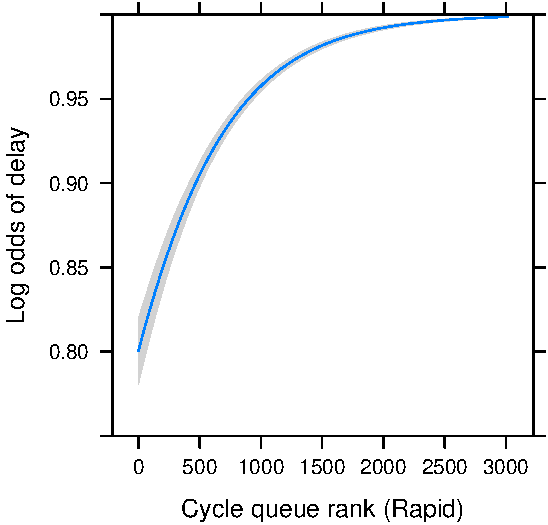
\includegraphics[width=0.43\textwidth,keepaspectratio]
		{chapters/chapter5/figures/rq3/cycle_queue_rank.pdf}
		\label{fig:cycle_rank}
	}

	\subfloat{
		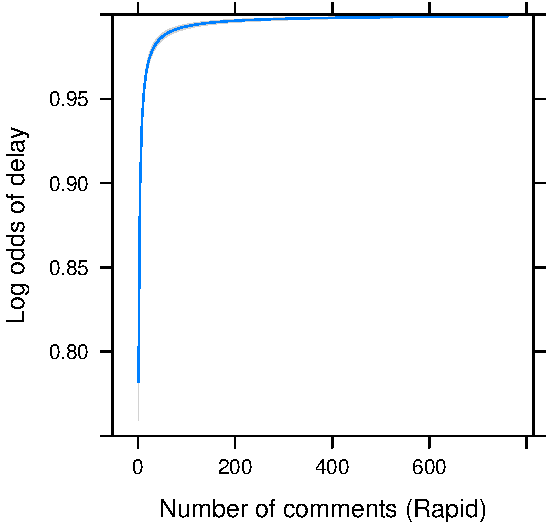
\includegraphics[width=0.43\textwidth,keepaspectratio]
		{chapters/chapter5/figures/rq3/comments.pdf}
		\label{fig:number_comments}
	}
	\caption{The relationship between metrics and delivery delay. The blue
		line shows the values of our model fit, whereas the grey
		area shows the 95\% confidence interval based on models fit to
		1,000 bootstrap samples. The parentheses indicate the
		release strategy to which the metric is related.
	}
\end{figure}

\begin{figure}[!]
	\centering
	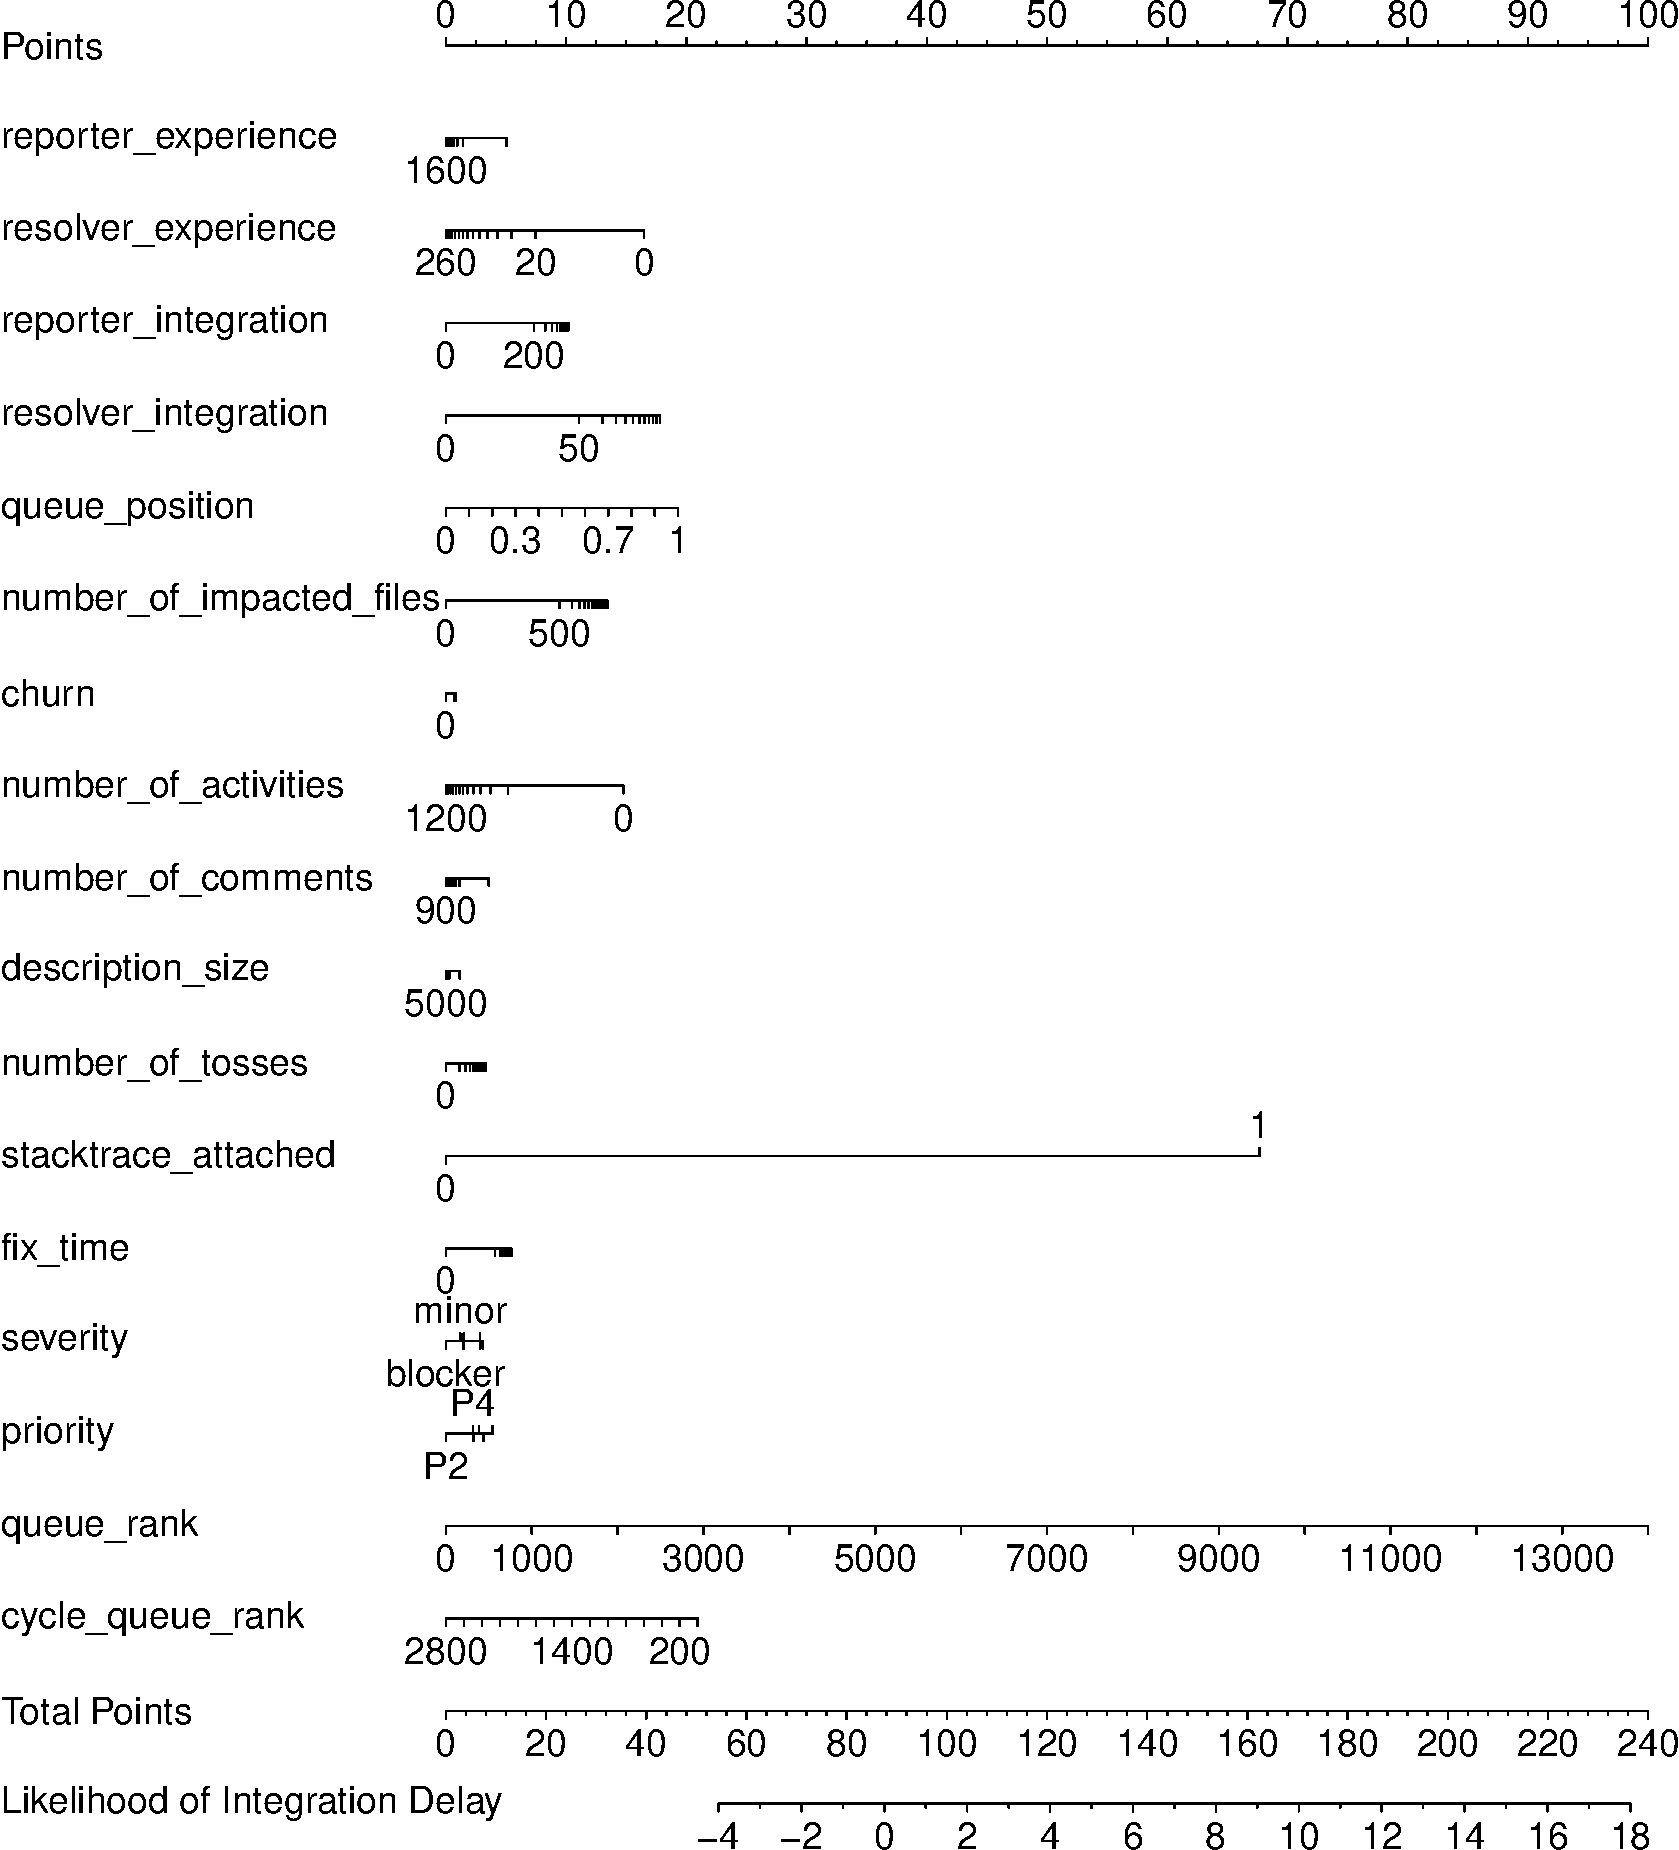
\includegraphics[width=0.90\textwidth,keepaspectratio]
	{chapters/chapter5/figures/rq3/nomogram_trad.pdf}
	\caption{Nomogram of our explanatory models for the traditional release cycle.}
	\label{fig:nomogram_trad}
\end{figure}

\begin{figure}[!]
	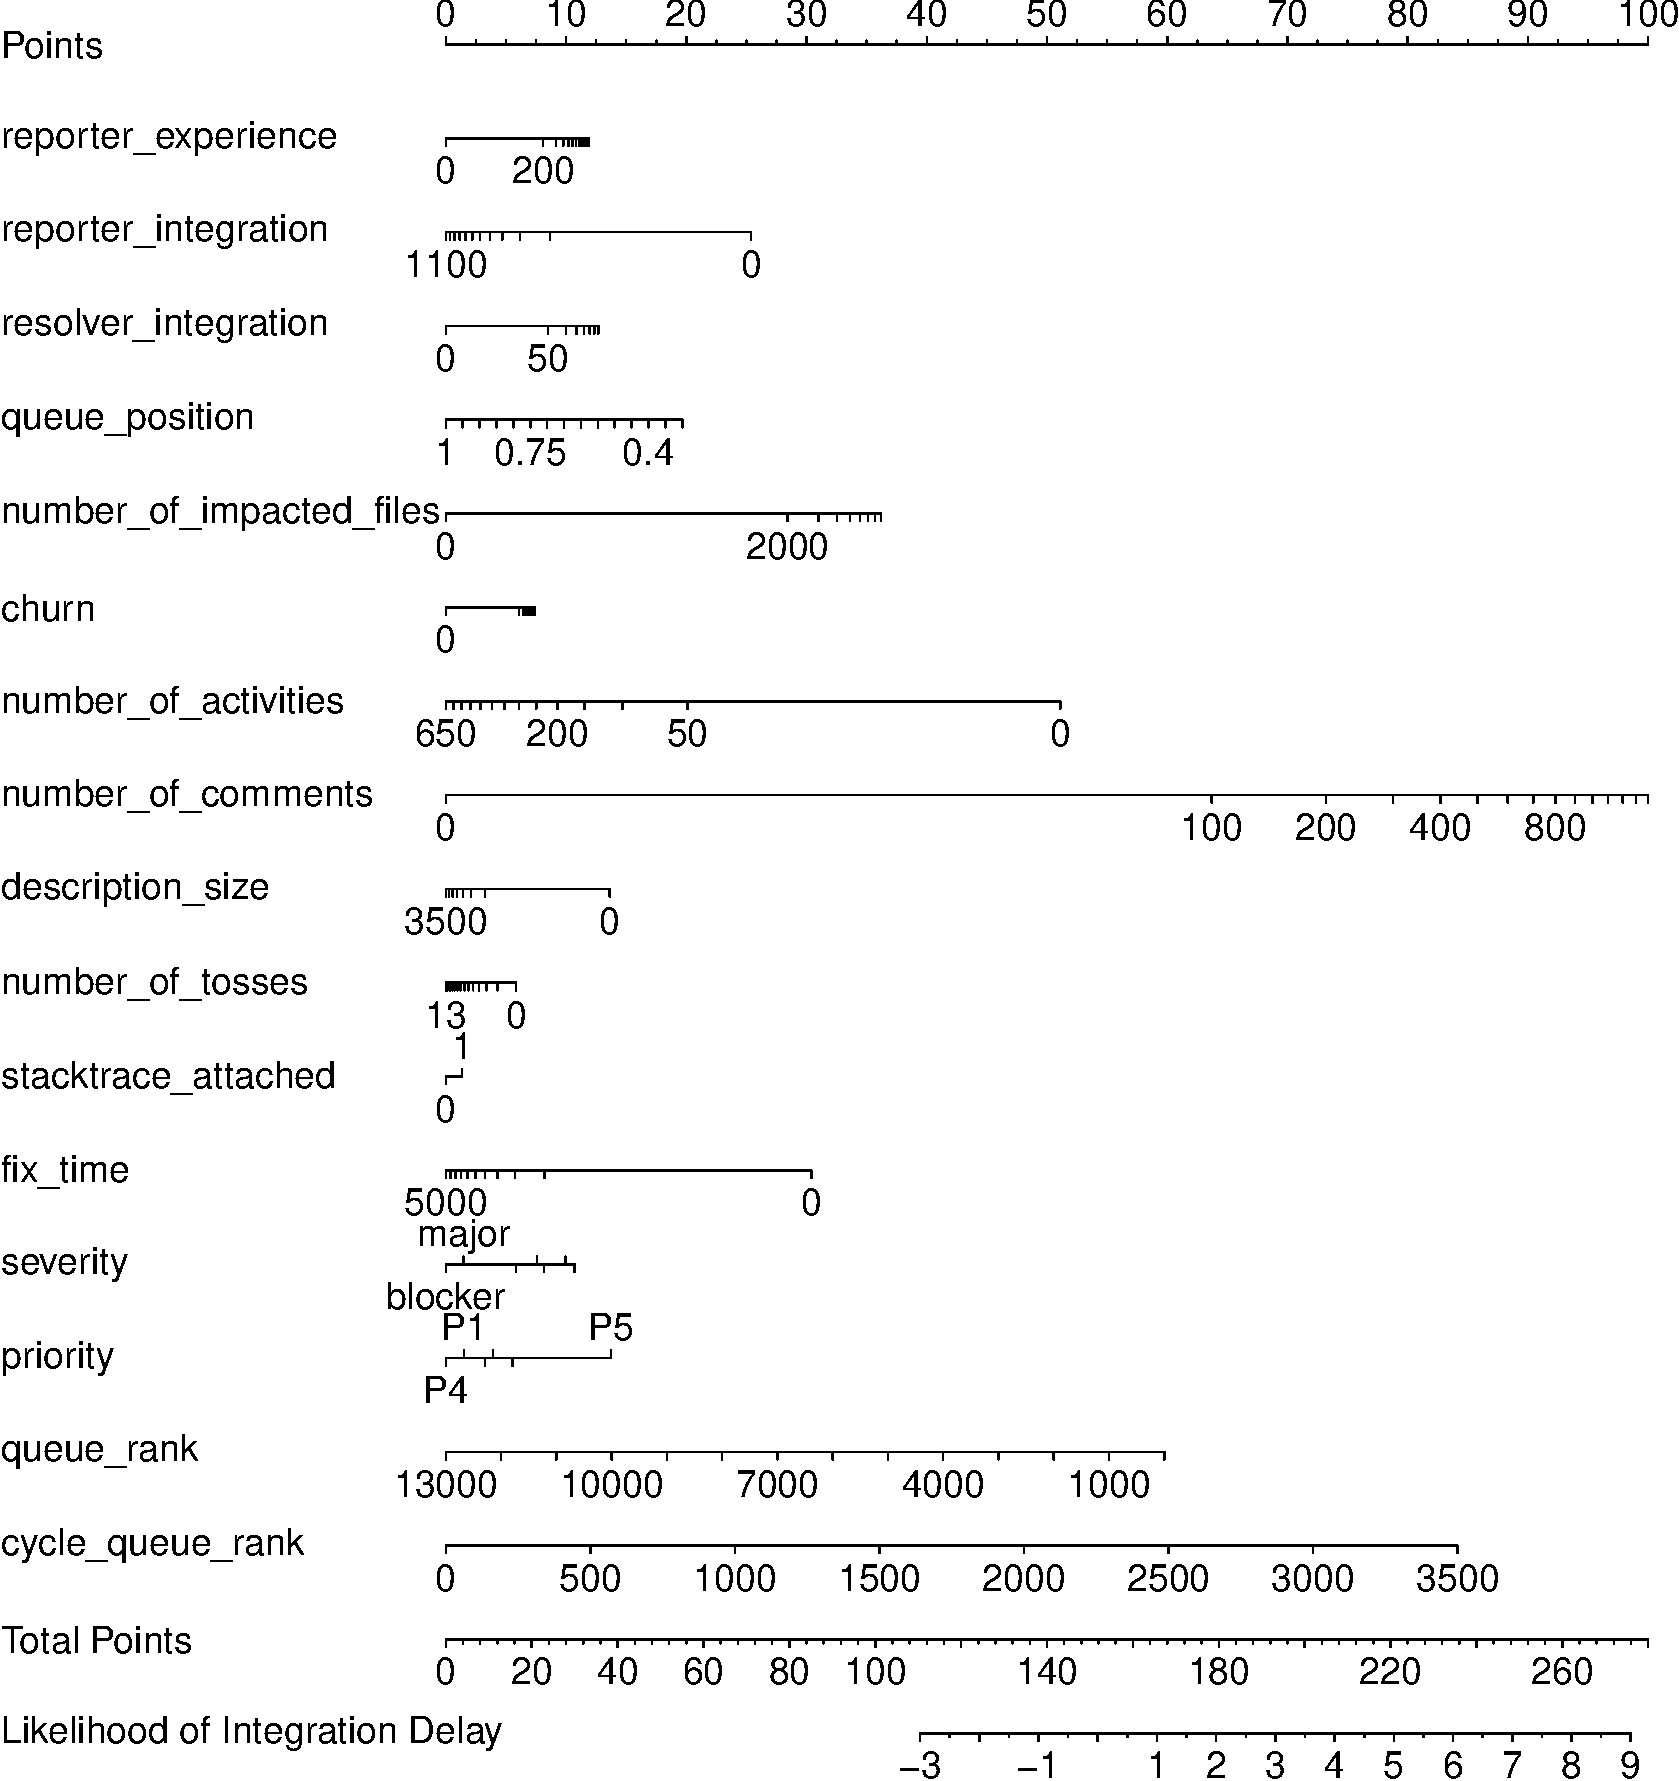
\includegraphics[width=0.90\textwidth,keepaspectratio]
	{chapters/chapter5/figures/rq3/nomogram_rapid.pdf}
	\caption{Nomogram of our explanatory models for the rapid release cycle.}
	\label{fig:nomogram_rapid}
\end{figure}

On the other hand, \textit{cycle queue rank} is the second-most important metric
in the models that we fit to the rapid release data. Cycle queue rank is the
moment when an issue is addressed in a given release cycle.
\hyperref[fig:cycle_rank]{Figure}~\ref{fig:cycle_rank} shows the relationship that cycle queue rank shares
with delivery delay. Our models reveal that the addressed issues in rapid
releases have a higher likelihood of being delayed if they were addressed later
than other addressed issues in the \textit{current release cycle}.
Interestingly, we observe that the most important metric in our rapid release
models is the \textit{number of comments}.
\hyperref[fig:number_comments]{Figure}~\ref{fig:number_comments}
shows the relationship that the \textit{number of comments} shares with
delivery delay. We observe that the greater the number of comments of an
addressed issue, the greater the likelihood of delivery delay. This result
corroborates the intuition that a lengthy discussion might be indicative of a
complex issue, which may be more likely to be delayed.

Moreover,
\hyperref[fig:nomogram_trad]{Figures}~\ref{fig:nomogram_trad}~and~\ref{fig:nomogram_rapid}
show the estimated effect of our metrics using
nomograms~\cite{iasonos2008build}. Indeed, our nomograms reiterate the large
impact of \textit{number of comments} (100 points) and \textit{cycle queue rank}
(84 points) in rapid releases, and the large impact of \textit{queue rank} (100
points) in traditional releases.  We also observe that \textit{stack trace
attached} has a large impact on traditional releases (68 points) despite not
being a significant contributor to the fit of our models (\cf
\hyperref[tbl:regression_models]{Table}~\ref{tbl:regression_models}). The large
impact shown in our nomogram for \textit{stack trace attached} is due to the
skewness of our data---only $5$ instances within the traditional release data
have the \textit{stack trace attached} set to true. Thus, \textit{stack trace
attached} cannot significantly contribute to the overall fit~of~our~models.

Another \textit{key} difference between traditional
and rapid releases is how addressed issues are prioritized for delivery.
Traditional releases are analogous to a queue in which the earlier an issue is
addressed, the lower its likelihood of delay. On the other hand, rapid
releases are analogous to a stack of cycles, in which the earlier an issue is
addressed in the current cycle, the lower its likelihood of delay.\\
\end{sloppypar}

\conclusionbox{Issues that are addressed early in the
	project backlog are less likely to be delayed in traditional releases.
	On the other hand, issues in rapid releases are queued up on a per
	release basis, in which issues that are addressed early in the release
cycle of the current release are less likely to be delayed.}
%\subsubsection*{Research Approach of Study 3} \label{ch5:approach_study3}
%
%\begin{figure}[t!]
%	\centering
%	\includegraphics[width=\columnwidth,keepaspectratio]
%	{chapters/chapter5/figures/rq1/issue_lifecycle.pdf}
%	\caption{A simplified life cycle of an issue.}
%	\label{fig:issue_lifecycle}
%\end{figure}
%
%\hyperref[fig:issue_lifecycle]{Figure}~\ref{fig:issue_lifecycle} shows a
%simplified life cycle of an issue, which includes the triaging phase ({\em t1}),
%the fixing phase ({\em t2}), and the integration phase ({\em t3}). We consider
%the last RESOLVED-FIXED status as the moment at which a particular issue was
%addressed (the fixed state in
%\hyperref[fig:issue_lifecycle]{Figure}~\ref{fig:issue_lifecycle}). The
%\textit{lifetime} of an issue is composed of all three phases (from \textit{new}
%to \textit{released}). For \hyperref[ch5:rq1]{RQ1}, we first observe the lifetime of the issues of
%traditional and rapid releases.  Next, we look at the time span of the
%\textit{triaging}, \textit{fixing}, and \textit{integration} phases within the
%lifetime of an issue. In \hyperref[ch5:rq2]{RQ2}, we group traditional and rapid releases into major
%and minor releases and study their delivery delays.
%
%We use beanplots~\cite{kampstra2008beanplot} to compare the distributions of our
%data. The vertical curves of beanplots summarize and compare the distributions
%of different datasets (see
%\hyperref[fig:delivery_delay]{Figure}~\ref{fig:delivery_delay}). The higher
%the frequency of data within a particular value, the thicker the bean is plotted
%at that particular value on the $y$ axis. We also use Mann-Whitney-Wilcoxon
%(MWW) tests~\cite{wilks2011statistical} and Cliff's delta effect-size
%measures~\cite{cliff1993dominance}. MWW tests are non-parametric tests of the
%\textit{null hypothesis} that two distributions come from the same population
%($\alpha=0.05$). On the other hand, Cliff's delta is a non-parametric
%effect-size measure to verify the difference in magnitude of one distribution compared
%to another distribution. The higher the value of the Cliff's delta,
%the greater the difference of values between distributions. For instance, if we
%obtain a significant $p$ value but a small Cliff's delta, this means that
%although two distributions do not come from the same population their 
%difference is not that large. A positive Cliff's delta indicates how much
%larger the values of the first distribution are, while a negative Cliff's delta
%indicates the inverse. Finally, we use the \textit{Median Absolute Deviation}
%(MAD) \cite{howell2005median,leys2013detecting} as a measure of the variation of
%our distributions. The MAD is the median of the \textit{absolute deviations}
%from one distribution's median. The higher the MAD, the greater is the variation
%of a distribution with respect to its median.
%
%\begin{table}[!t]
%	\footnotesize
%	\caption{Metrics that are used in our explanatory models (Reporter, Resolver,
%		and Issue families).
%	\label{tbl:factors1}}
%	\centering
%		\begin{tabular}{rp{2cm}lp{9cm}}
%			\hline
%			\multicolumn{1}{c}{\textbf{Family}} &
%			\multicolumn{1}{c}{\textbf{Metrics}} & \multicolumn{1}{c}{\textbf{Value}} &
%			\multicolumn{1}{c}{\textbf{Definition (d)$\vert$Rationale (r)}}
%			\\ \hline
%			\multicolumn{ 1}{r}{\textbf{Reporter}} & Experience & Numeric & 
%			\begin{tabular}{p{8.7cm}}
%				\textbf{d:} the number of previously delivered issues that were reported by
%				the reporter of a particular addressed issue.  \\ \hline 
%				\textbf{r:} The greater the experience of the reporter the
%				higher the quality of his/her reports and the
%				solution to his/her reports might be delivered
%				more quickly~\cite{shihab2010predicting}.
%			\end{tabular}
%			\\ \cline{2- 4}
%			\multicolumn{ 1}{r}{} & Reporter integration & Numeric &
%			\begin{tabular}{p{8.7cm}}
%				\textbf{d:} The median in days of the previously delivered addressed issues
%				that were reported by a particular reporter.
%				\\ \hline 
%				\textbf{r:} If a particular reporter usually reports issues that are
%				delivered quickly, his/her future reported issues might be delivered
%				quickly as well.
%			\end{tabular}
%			\\ \hline
%			\multicolumn{ 1}{r}{\textbf{Resolver}} & Experience & Numeric & 
%			\begin{tabular}{p{8.7cm}}
%				\textbf{d:} the number of previously delivered addressed issues that were
%				addressed by the resolver of a particular
%				addressed issue. We consider the collaborator
%				that changed the status of an issue to
%				RESOLVED-FIXED as the resolver of that issue. \\ \hline 
%				\textbf{r:} The greater the experience of the resolver, the
%				greater the likelihood that his/her code will be
%				delivered faster~\cite{shihab2010predicting}.
%			\end{tabular}
%			\\ \cline{2- 4}
%			\multicolumn{ 1}{r}{} & Resolver integration & Numeric &
%			\begin{tabular}{p{8.7cm}}
%				\textbf{d:} The median in days of the previously delivered addressed issues
%				that were addressed by a particular resolver.
%				\\ \hline 
%				\textbf{r:} If a particular resolver usually address issues that are
%				delivered quickly, his/her future addressed issues might be delivered
%				quickly as well.
%			\end{tabular}
%			\\ \hline
%			\multicolumn{ 1}{r}{\textbf{Issue}} & Stack trace attached & Boolean &
%			\begin{tabular}{p{8.7cm}}
%				\textbf{d:} We verify if the issue report has a stack trace attached in its description. \\ \hline 
%				\textbf{r:} A stack trace attached may provide useful information regarding
%				the cause of the issue, which may quicken the integration of
%				the addressed issue~\cite{schroter2010stack}. 
%			\end{tabular}
%			\\ \cline{2- 4}
%			\multicolumn{ 1}{r}{} & Severity & Nominal &
%			\begin{tabular}{p{8.7cm}}
%				\textbf{d:} The severity level of the issue report. Issues with higher
%				severity levels (\eg blocking) might be delivered faster than other issues.
%				\\ \hline 
%				\textbf{r:} Panjer observed that the severity of an issue has a large effect
%				on its time to be addressed in the Eclipse project~\cite{Panjer2007}.
%			\end{tabular}
%			\\ \cline{2- 4}
%			\multicolumn{ 1}{r}{} & Priority & Nominal &
%			\begin{tabular}{p{8.7cm}}
%				\textbf{d:} The priority level of the issue report. Issues with higher
%				priority levels (\eg P1) might be delivered faster than other issues.
%				\\ \hline 
%				\textbf{r:} Higher priority issues will likely be delivered before lower
%				priority issues.
%			\end{tabular}
%			\\ \cline{2- 4}
%			\multicolumn{ 1}{r}{} & Description size & Numeric &
%			\begin{tabular}{p{5.6cm}}
%				\textbf{d:} The number of words in the description of the issue. 
%				\\ \hline 
%				\textbf{r:} Issues that are well described might be more easy to integrate
%				than issues that are difficult to understand.
%			\end{tabular}
%			\\ \hline
%		\end{tabular}
%\end{table}
%
%\begin{figure}[t!]
%	\centering
%	\includegraphics[width=\columnwidth,keepaspectratio]
%	{chapters/chapter5/figures/rq3/model_construction.pdf}
%	\caption{Overview of the process that we use to build our explanatory models.}
%	\label{fig:model_construction}
%\end{figure}
%
%\begin{table}[!t]
%	\footnotesize
%	\caption{Metrics that are used in our explanatory models (Project family).
%	\label{tbl:factors2}}
%	\centering
%		\begin{tabular}{rp{2cm}lp{9cm}}
%			\hline
%			\multicolumn{1}{c}{\textbf{Family}} &
%			\multicolumn{1}{c}{\textbf{Metrics}} & \multicolumn{1}{c}{\textbf{Value}} &
%			\multicolumn{1}{c}{\textbf{Definition (d)$\vert$Rationale (r)}}
%			\\ \hline
%			\multicolumn{ 1}{r}{\textbf{Project}} & Queue rank & Numeric &
%			\begin{tabular}{p{8.7cm}}
%				\textbf{d:} A rank number that represents the
%				moment at which an issue is
%				addressed compared to other addressed issues in the backlog. For instance,
%				in a backlog that contains $500$ issues, the first addressed issue has
%				a rank of~1, while the last addressed issue has
%				a rank of 500.
%				\\ \hline 
%				\textbf{r:} An issue with a high \textit{queue rank} is a recently
%				addressed issue. An addressed issue might be delivered faster/slower
%				depending of its rank.
%			\end{tabular}
%			\\ \cline{2- 4}
%			\multicolumn{ 1}{r}{} & Cycle queue rank & Numeric &
%			\begin{tabular}{p{8.7cm}}
%				\textbf{d:} A rank number that represents the
%				moment at which an issue is
%				addressed compared to other addressed issues of the same release cycle. For
%				example, in a release cycle that contains $300$ addressed issues, the first
%				addressed issue has a rank of $1$, while the
%				last one has a rank of $300$.
%				\\ \hline 
%				\textbf{r:} An issue with a high \textit{cycle queue rank} is a recently
%				addressed issue compared to the others of the same release cycle. An issue
%				addressed close to the upcoming release might be delivered faster.
%			\end{tabular}
%			\\ \cline{2- 4}
%			\multicolumn{ 1}{r}{} & Queue position & Numeric &
%			\begin{tabular}{p{8.7cm}}
%				\textbf{d:} $\frac{\text{queue rank}}{\text{all addressed issues}}$. The
%				\textit{queue rank} is divided by all the issues that are addressed by the
%				end of the next release. A \textit{queue position} close to 1 indicates that the
%				issue was addressed recently compared to others in the backlog.
%				\\ \hline 
%				\textbf{r:} An addressed issue
%				might be delivered faster/slower depending of its position.
%			\end{tabular}
%			\\ \cline{2- 4}
%			\multicolumn{ 1}{r}{} & Cycle queue position & Numeric &
%			\begin{tabular}{p{8.7cm}}
%				\textbf{d:} $\frac{\text{cycle queue rank}}{\text{addressed issues of the
%				current cycle}}$. The \textit{cycle queue rank} is divided by all of the
%				addressed issues of the release cycle. A \textit{cycle
%				queue position} close to 1 indicates that the issue was addressed recently
%				in the release cycle.
%				\\ \hline 
%				\textbf{r:}  An issue addressed close
%				to a upcoming release might be delivered faster. 
%			\end{tabular}
%			\\ \hline
%		\end{tabular}
%\end{table}
%
%\begin{table}[!t]
%	\footnotesize
%	\caption{Metrics that are used in our explanatory models (Process family).
%	\label{tbl:factors3}}
%	\centering
%		\begin{tabular}{rp{2cm}lp{9cm}}
%			\hline
%			\multicolumn{1}{c}{\textbf{Family}} &
%			\multicolumn{1}{c}{\textbf{Metrics}} & \multicolumn{1}{c}{\textbf{Value}} &
%			\multicolumn{1}{c}{\textbf{Definition (d)$\vert$Rationale (r)}}
%			\\ \hline
%			\multicolumn{ 1}{r}{\textbf{Process}} & Number of Impacted Files & Numeric & 
%			\begin{tabular}{p{8.7cm}}
%				\textbf{d:} The number of files that are linked to an issue report. \\ \hline 
%				\textbf{r:} A delivery delay might be
%				related to a high number of impacted files 
%				because more effort would be required to properly integrate the modifications 
%				\cite{Jiang2013}. 
%			\end{tabular}
%			\\ \cline{ 2- 4}
%			\multicolumn{ 1}{r}{} & Churn & Numeric &
%			\begin{tabular}{p{8.7cm}}
%				\textbf{d:} The sum of added lines plus the sum
%				of deleted lines to address the issue.\\ \hline 
%				\textbf{r:} A higher churn suggests that a great amount of work was required
%				to address the issue, and hence, verifying the impact of integrating the
%				modifications may also be difficult~\cite{Jiang2013,Nagappan2005}.
%			\end{tabular}
%			\\ \cline{2- 4}
%			\multicolumn{ 1}{r}{} & Fix time & Numeric &
%			\begin{tabular}{p{8.7cm}}
%				\textbf{d:} Number of days between the date when
%				the issue was
%				triaged and the
%				date that it was addressed~\cite{Giger2010}. \\ \hline 
%				\textbf{r:} If an issue is addressed quickly, it may have a better chance to
%				be delivered faster.
%			\end{tabular}
%			\\ \cline{ 2- 4}
%			\multicolumn{ 1}{r}{} & Number of activities & Numeric &
%			\begin{tabular}{p{8.7cm}}
%				\textbf{d:} An activity is an entry in the issue's history. \\ \hline 
%				\textbf{r:} A high number of activities might indicate that much work was
%				required to address the issue, which may impact the integration of the
%				issue into a release~\cite{Jiang2013}.
%			\end{tabular}
%			\\ \cline{ 2- 4}
%			\multicolumn{ 1}{r}{} & Number of comments & Numeric & 
%			\begin{tabular}{p{8.7cm}}
%				\textbf{d:} The number of comments of an issue report. \\ \hline 
%				\textbf{r:} A large number of comments might indicate the importance of an
%				issue or the difficulty to understand it~\cite{Giger2010}, which might
%				impact the delivery delay~\cite{Jiang2013}.
%			\end{tabular}
%			\\ \cline{ 2- 4}
%			\multicolumn{ 1}{r}{} & Interval of comments & Numeric &
%			\begin{tabular}{p{8.7cm}}
%				\textbf{d:} The sum of the time intervals (hour) between
%				comments divided by the total number of comments of an issue report. \\ \hline 
%				\textbf{r:} A short \textit{interval of comments} indicates that an intense
%				discussion took place, which suggests that the issue is important. Hence,
%				such an issue may be delivered faster.   
%			\end{tabular}
%			\\ \cline{ 2- 4}
%			\multicolumn{ 1}{r}{} & Number of tosses & Numeric &
%			\begin{tabular}{p{8.7cm}}
%				\textbf{d:} The number of times that the assignee has changed. \\ \hline 
%				\textbf{r:} Changes in the issue assignee might indicate that more than one
%				developer have worked on the issue. Such issues may be more difficult to
%				integrate, since different expertise from different developers might 
%				be required~\cite{Jeong2009,Jiang2013}.  
%			\end{tabular}
%			\\ \hline
%		\end{tabular}
%\end{table}
%
%For \hyperref[ch5:rq3]{RQ3}, we build explanatory models (\ie logistic
%regression models) for the traditional and rapid releases data using the metrics
%that are presented in
%\hyperref[tbl:factors1]{Tables}~\ref{tbl:factors1},~\ref{tbl:factors2}, and
%\ref{tbl:factors3}. We model our response variable $Y$ as $Y=1$ for addressed
%issues that are delayed, \ie had their delivery prevented in at least one
%release\cite{costa2014empirical} and $Y=0$ otherwise. Hence, our models are
%intended to explain why a given addressed issue has a delayed delivery (\ie
%$Y=1$).
%
%We follow the guidelines of Harrell~Jr.~\cite{harrell2001regression} for
%building explanatory regression models.
%\hyperref[fig:model_construction]{Figure}~\ref{fig:model_construction} provides
%an overview of the process that we use to build our models. First, we estimate
%the budget of degrees of freedom that we can spend on our models while having a
%low risk of overfitting (\ie producing a model that is too specific to the
%training data to be useful when applied to other unseen data). Second, we check for
%metrics that are highly correlated using Spearman rank correlation tests
%$(\rho)$ and we perform a redundancy analysis to remove any redundant metrics
%before building our explanatory models. 
%
%We then assess the fit of our models using the ROC area and the Brier score. The
%ROC area is used to evaluate the degree of discrimination that is achieved by
%a model. The ROC values range between 0 (worst) and 1 (best). An area greater
%than 0.5 indicates that the explanatory model outperforms na\"{i}ve random
%guessing models. The Brier score is used to evaluate the accuracy of
%probabilistic predictions. This score measures the mean squared difference
%between the probability of delay assigned by our models for a particular issue
%$I$ and the actual outcome of $I$ (\ie whether $I$ is actually delayed or not).
%Hence, the lower the Brier score, the more accurate the probabilities that are
%produced by a model.
%
%Next, we assess the stability of our models by computing the
%\textit{optimism-reduced} ROC area and Brier score~\cite{efron1986biased}. The
%optimism of each metric is computed by selecting a bootstrap sample to
%fit a model with the same degrees of freedom of the original model. The model
%that is trained using the bootstrap sample is applied both on the bootstrap and original
%samples (ROC and Brier scores are computed for each sample). The optimism is the
%difference in the ROC area and Brier score of the bootstrap sample and original
%sample. This process is repeated 1,000 times and the average optimism is
%computed. Finally, we obtain the \textit{optimism-reduced} scores by subtracting
%the average optimism from the initial ROC area and Brier score
%estimates~\cite{efron1986biased}.
%
%We evaluate the impact of each metric on the fitted models using
%Wald $\chi^2$ maximum likelihood tests. The larger the $\chi^2$ value, the
%larger the impact that a particular metric has on our explanatory models'
%performance. We also study the relationship that our metrics 
%share with the likelihood of delivery delay. To do so, we plot the change in
%the estimated probability of delay against the change in a given metric
%while holding the other metrics constant at their median values using the
%\code{Predict} function of the \code{rms} package~\cite{harrell2001regression}. 
%
%We also plot nomograms~\cite{iasonos2008build,harrell2001regression} to evaluate
%the impact of the metrics in our models. Nomograms are user-friendly charts that
%visually represent explanatory models. For instance,
%\hyperref[fig:nomogram_trad]{Figure}~\ref{fig:nomogram_trad} shows the nomogram
%of the model that we fit for the rapid release data. The higher the number of
%points that are assigned to an explanatory metric on the $x$ axis (\eg 100
%points are assigned to \textit{comments} in rapid releases), the larger the
%effect of that metric in the explanatory model. We compare which metrics are
%more important in both traditional and rapid releases in order to better
%understand the differences between these release strategies.
%
%
%\subsection{Methodology of Study 4}
%
%In this study, we qualitatively analyze the delivery delay phenomena by
%surveying and interviewing the team members of our subject projects.
%
%\subsection{Subjects of Study 4}
%
%We analyze the Firefox, ArgoUML, and Eclipse (JDT) projects. We naturally choose
%these projects, since this qualitative study is intended to complement our prior
%quantitative analyses that we performed in those projects. We provide a brief
%description of each subject project below (we have already provided a detailed
%description in \hyperref[ch4:sec:subjects]{Section}~\ref{ch4:sec:subjects}).
%
%ArgoUML is an open source UML modeling tool. ArgoUML provides support for all of
%the UML 1.4 diagrams. At the time that we perform this study, ArgoUML was
%downloaded 80,000 times worldwide.\smartfoot{\url{http://argouml.tigris.org}}
%ArgoUML uses the IssueZilla ITS to record its issue
%reports.\smartfoot{\url{http://argouml.tigris.org/project_bugs.html}}
%
%Eclipse is a popular {\em Integrated Development Environment} (IDE) that is
%famous for its support for the Java programming
%language.\smartfoot{\url{https://eclipse.org/}} We study the {\em Java
%Development Tools} (JDT) project of the Eclipse
%Foundation.\smartfoot{\url{https://projects.eclipse.org/projects/eclipse.jdt}}
%The JDT project provides the Java perspective for the Eclipse IDE, which
%includes a number of views, editors, wizards, and builders. 
%
%ArgoUML and Eclipse (JDT) adopt a traditional release cycle when compared to the
%Firefox project. For instance, the median duration of release cycles that we
%study for the ArgoUML and Eclipse (JDT) projects are 180 and 112 days,
%respectively (see \hyperref[ch:study12]{Chapter}~\ref{ch:study12}). While we are
%able to study the perceived impact of the shift between release strategies when
%surveying the participants of the Firefox project, we study the opinion of the
%ArgoUML and Eclipse participants about how that impact would be on their
%projects.
%
%\subsection{Data collection for Study 4}\label{ch5:datacollection2}
%
%\begin{table}[t!]
%	\centering
%	\footnotesize
%	\caption{\textbf{Survey questions (excerpt).} Each horizontal line indicates a page break.
%	\label{tbl:survey}}
%		\begin{tabular}{p{0.95\textwidth}}
%			\hline 
%			\textbf{1.} For how long have you been developing software? {\em (dropdown)}\tabularnewline
%			\textbf{2.} For how long have you worked in the (Firefox/ArgoUML/Eclipse) project?
%			{\em (dropdown)}\tabularnewline
%			\textbf{3.} How would you describe your roles in the software development of
%			the Firefox/ArgoUML/Eclipse project? (e.g., developer, tester, release manager, etc.)
%			{\em (text box)}\tabularnewline
%			\textbf{4.} In your opinion, what motivates a development team to shift from
%			a traditional release cycle (e.g., a release every 9 to 18 months)
%			to a rapid release cycle (e.g., a release every 6
%			weeks)? {\em (text box)}\tabularnewline
%			\textbf{5.} In this survey, we consider that an issue is completed when it
%			is implemented and tested, i.e., it is ready to be delivered. Do
%			you remember an issue that the development team completed work on,
%			but was not delivered to end users through the next possible release?
%			Can you tell us what caused the delivery delay of this issue in your
%			opinion? {\em (text box)}\tabularnewline
%			\textbf{6.} In your experience, how common are the cases in which completed
%			issues (issues that are implemented and tested) are omitted from the
%			next possible release?\tabularnewline
%			\textbf{7.} Who decides when a completed issue is delivered into an official
%			release in your team? {\em (text box)}\tabularnewline
%			\textbf{8.} In your opinion, when is the delivery of a completed issue to the
%			end user considered to be delayed in your project? {\em (text box)}\tabularnewline
%			\hline 
%			\textbf{9.} In your opinion, is it frustrating to users when a completed issue
%			skips one or more releases? Why? {\em (text box)}\tabularnewline
%			\textbf{10.} Is it frustrating for the team members when a completed issue
%			skips one or more releases? Why? {\em (text box)}\tabularnewline
%			\hline 
%			\textbf{11.} Assuming that an issue is completed today (implementation and
%			testing are completed), what reasons can you think of for the issue
%			not to be delivered to end users in the next release? {\em (text box)}\tabularnewline
%			\hline 
%			\textbf{12.} What can team members do to avoid the delivery delay of completed
%			issues? {\em (text box)}\tabularnewline
%			\textbf{13.} To what extent do you agree that the characteristics listed in
%			the table below are related to the delivery delay of a
%			completed issue?\\
%			- The reporter of an addressed issue, the resolver of an
%			addressed issue, the priority level, the severity level,
%			number of comments, number of modified files, number of
%			lines of code, the time at which an issue was addressed
%			during the release cycle.
%			{\em (5-point Likert scale for each option)}\tabularnewline
%			\hline 
%			\textbf{14-Firefox.} Have you worked in both traditional and rapid release cycles of
%			the Firefox project? {\em (yes/no)}\tabularnewline
%			\textbf{15-Firefox.} In your opinion, how much impact does a rapid release cycle have
%			on the time to deliver completed issues for end users?
%			{\em (text box)}\tabularnewline
%			\textbf{16-Firefox.} Did your project evaluate the shift to rapid release cycles? If
%			so, how? {\em (text box)}\tabularnewline
%			\textbf{14-Others.} Do you have experience working on a
%			rapid release cycle in any other project? {\em (yes/no)}\tabularnewline
%			\textbf{15-Others.} In your opinion, what would be the
%			impact of shifting to a rapid release cycle (e.g., a
%			release every 6 weeks rather than a release every 9 to
%			18 months) on the delay to deliver completed issues, in
%			your project? {\em (text box)}\tabularnewline
%			\textbf{16-Others.} If your project had shifted from a
%			traditional to a rapid release cycle, how would you
%			evaluate if this shift benefited your project? {\em (text box)}
%		\end{tabular}
%\end{table}
%
%To collect the data to perform our qualitative study, we design a web-based
%survey that was sent to 780 participants of the Firefox, Eclipse (JDT), and
%ArgoUML projects. We sent our survey to 513 Firefox, 184 Eclipse (JDT), and 83
%ArgoUML participants. We gather developer e-mails from the respective
%developer mailing list archives of the subject projects. We consider e-mail
%addresses from messages that were sent in the past 4 years. To
%encourage participation, we provided gift cards to a random subset of the
%respondents who answered all of the questions of our surveys.
%
%Our survey is based on the two major {\em themes} that are investigated in this
%thesis. The first {\em theme} is about
%delivery delay in general, while the second {\em theme} is focused on the
%impact of switching to a rapid release cycle on the delivery delay (see
%\hyperref[fig:thesis_overview]{Figure}~\ref{fig:thesis_overview}). In
%\hyperref[tbl:survey]{Table}~\ref{tbl:survey}, we highlight a subset of the
%questions of our survey. Each horizontal line represents a page break in the
%survey. Our complete surveys are available in
%\hyperref[appendix:a]{Appendices}~\ref{appendix:a},~\ref{appendix:b},~and~\ref{appendix:c}.
%The first three questions collect demographic information. Questions \#5-13
%belong to the general delivery delay {\em theme}, while questions \#4,
%\#14-16 belong to the impact of switching to a rapid release cycle {\em theme}.
%We placed one question of the second {\em theme} early in the survey to mitigate
%bias in the responses about the motivation to switch to a rapid release cycle.
%Finally, questions \#14-16 are different for the Firefox project, since the
%other projects did not shift from a traditional to a rapid release cycle. 
%
%In total, we receive 37 responses (5\% response rate), of which 25 responses
%come from Firefox participants, 9 from Eclipse participants, and 3 from ArgoUML
%participants. We also conduct follow-up interviews with four of the Firefox
%participants to gather deeper insights into their responses. Our interviews are
%semi-structured and our goal was to clarify the responses of our survey and
%collect more details about specific cases of delivery delays for addressed
%issues.  
%
%\subsection{Research Approach of Study~4}
%
%Given the exploratory nature of our qualitative analysis, we use methods from
%{\em Grounded Theory}~\cite{groundtheorybook}. The author of this thesis and
%co-author~\#1 independently conduct three sessions of open coding of the
%responses to open-ended questions (one session for each RQ). In the following,
%the codes that were generated are shared and merged into a new set of codes. The
%co-author~\#2 reviews the set of codes and adds additional entries to the final
%set of codes.  At the end of the process, we achieve 175 unique codes. Finally,
%we used axial coding to find higher level conceptual themes to answer our RQs.
%
%\begin{table}
%	\footnotesize
%	\centering
%	\caption{Participant range per subject project.
%		\label{tbl:participants}
%	}
%	\begin{tabular}{lc}
%		\hline 
%		\textbf{Project} & \textbf{Participant range}\tabularnewline
%		\hline 
%		\hline 
%		Firefox & F01--F25\tabularnewline
%		\hline 
%		Eclipse & E26--E34\tabularnewline
%		\hline 
%		ArgoUML & A35--A37\tabularnewline
%		\hline 
%	\end{tabular}
%\end{table}
%
%When reporting the results of \hyperref[ch5:rq4]{RQ4}-\hyperref[ch5:rq6]{RQ6},
%we indicate in superscript the number of participants that mentioned a
%particular code that emerged during the qualitative analysis. These numbers do
%not necessarily indicate the importance of a given code, since they were coded
%based on the received responses rather than scored by participants. Also, we
%mention quotes from the interviews when necessary to provide more detail about
%the results and to allow for traceability through links to raw data. Finally,
%\hyperref[tbl:participants]{Table}~\ref{tbl:participants} shows the IDs of the
%participants that we use while reporting results.
%
%Finally, we also perform quantitative analyses of the responses to Likert-scale
%questions. First, we check if the factors that are listed in {\em question~\#13}
%are significantly different using the ranks (responses) that are assigned to
%each factor. We use a Kruskal Wallis test~\cite{kruskal1952use} to check if
%there is a statistically significant difference between the ranks assigned to
%the factors. The Kruskal Wallis test is the non-parametric equivalent of the
%ANOVA test~\cite{fisher1925statistical} to check if there are statistically
%significant differences when comparing three or more distributions. Since
%Kruskal Wallis does not indicate which factor has statistically different values
%with respect to others, we use the Dunn test~\cite{dunn1964multiple} to perform
%specific comparisons. For example, the Dunn test indicates if the ranks that are
%assigned to the {\em number of comments} metric are statistically different when
%compared to the ones that are assigned to the {\em number of modified files}
%metric. We use the Bonferroni correction~\cite{dunn1961multiple} on the obtained
%$p$ values to account for the multiple comparisons that we perform between each
%of the factors that are listed in {\em question~\#13}. 
%
%Additionally, we correlate the ranks that are assigned to the factors in {\em
%question~\#13} with the experience of the participants ({\em question~\#1}). To
%do that, we use Spearman rank {$\rho$} correlation~\cite{spearman1904proof},
%which is used to measure the statistical dependence between the ranks of two
%variables. Finally, we also correlate the experience of the participants with
%the perception of the frequency of delivery delay that happens in the studied
%projects ({\em question~\#6}).
%
%\subsection{Exploratory Analysis}\label{subsubsec:exploratory}
%
%\begin{figure}
%	\centering
%	\includegraphics[width=0.80\textwidth,keepaspectratio] 
%	{chapters/chapter5/figures/demographic_experience.pdf}
%	\caption{Software development experience of the participants.}
%	\label{fig:demographics_experience}
%\end{figure}
%We present a exploratory analysis of the data that we collect from the responses
%of the participants.
%\hyperref[fig:demographics_experience]{Figure}~\ref{fig:demographics_experience}
%shows the experience of the participants. We collect this data from {\em
%question~\#1}. The options range from ``0 years'' to ``10 or more years''. We
%observe that 62\% ($\frac{23}{37}$) of the participants have ``10 or more
%years'' of software development experience. 
%\begin{figure}
%	\centering
%	\includegraphics[width=0.80\textwidth,keepaspectratio] 
%	{chapters/chapter5/figures/demographic_experience_project.pdf}
%	\caption{Development experience of the participants in the
%	respective project.}
%	\label{fig:demographics_experience_project}
%\end{figure}
%Furthermore,
%\hyperref[fig:demographics_experience_project]{Figure}~\ref{fig:demographics_experience_project}
%shows the experience of the participants related to the specific project that
%they are representing. We collect this data from {\em question~\#2} and the
%options range from ``0 years'' to ``5 or more years''. 51\%  ($\frac{19}{37}$)
%of the participants have 4 or more years of experience. 
%\begin{figure}
%	\centering
%	\includegraphics[width=0.80\textwidth,keepaspectratio] 
%	{chapters/chapter5/figures/demographic_rapid_releases.pdf}
%	\caption{Experience of the participants with respect to rapid release
%	cycles.}
%	\label{fig:demographics_rapid_releases}
%\end{figure}
%Moreover,
%\hyperref[fig:demographics_rapid_releases]{Figure}~\ref{fig:demographics_rapid_releases}
%shows how many participants have experience in working on rapid release cycles
%({\em question~\#14}). We note that 57\% ($\frac{21}{37}$) of the participants
%have some experience with rapid release cycles.
%\begin{figure}
%	\centering
%	\includegraphics[width=0.80\textwidth,keepaspectratio] 
%	{chapters/chapter5/figures/roles_demographics.pdf}
%	\caption{An overview of the roles of the participants. One participant
%	may have more than one role.}
%	\label{fig:roles_demographics}
%\end{figure}
%\hyperref[fig:roles_demographics]{Figure}~\ref{fig:roles_demographics} shows the
%team roles that the participants classified themselves as ({\em question~\#3}).
%The majority of the participants consider themselves as ``developers'' and
%``testers''. Since one participant can occupy several roles, the numbers that
%are shown in
%\hyperref[fig:roles_demographics]{Figure}~\ref{fig:roles_demographics} represent
%the frequency that a role was cited rather than the number of participants.
%\begin{figure}
%	\centering
%	\includegraphics[width=0.80\textwidth,keepaspectratio] 
%	{chapters/chapter5/figures/delay_perception.pdf}
%	\caption{Participants' perception on how frequent is delivery delay. The data is grouped by proportions of
%		how many addressed issues are included in the next possible
%		release. This data refers to the responses to {\em question~\#6}.}
%	\label{fig:delay_perception}
%\end{figure}
%Finally, we observe that the majority of the participants perceive delivery delay as an unusual event rather than
%typical (see \hyperref[fig:delay_perception]{Figure}~\ref{fig:delay_perception}). For instance, 14 of the Firefox
%participants think that 90\% of the issues are included in the next possible release.
%
%In our analyses to answer \hyperref[ch5:rq4]{RQ4}-\hyperref[ch5:rq6]{RQ6}, we
%attempt to correlate the rating of factors that are provided in {\em
%question~\#13} with the data that is presented in this preliminary analysis.
%
%\subsection{Research Questions of Study~4}
%
%We present the three research questions that are addressed in
%\hyperref[st:study4]{Study}~\ref{st:study4} below.
%
%
%\subsubsection*{\textit{RQ4: What are developers' perceptions as to why integration
%delays occur?}}\label{ch5:rq4}
%
%\subsubsection*{RQ4: Motivation}
%
%To the best of our knowledge, there is no prior work that qualitatively studies
%delivery delay. Qualitative studies are important to detect phenomena that are
%difficult to uncover quantitatively. Our goal in this RQ is to better understand
%{\em \underline{why}} delivery delays happen. This investigation is a starting
%point to reveal new ways of mitigating delivery delays.\\
%
%\subsubsection*{RQ4: Results}
%
%\begin{sloppypar}
%Our findings about developers' perceptions of the causes of delivery delay is
%divided into the following themes: {\em (i) development activities}, {\em (ii)
%decision making}, {\em (iii) risk}, {\em (iv) frustration}, and {\em (v) team
%collaboration}. After discussing each theme below, we present a quantitative
%analysis of the factors that can impact delivery delay using the responses to
%{\em question~\#13} (see our \hyperref[ch5:datacollection2]{data collection}
%process).\\ 
%
%\noindent\textit{\textbf{Theme~1---Development activities.}}\theme{th:1} 
%The number of tests that should be executed was a recurrent theme among
%participants. For instance, several participants stated that {\em additional
%testing}$^{(12)}$ should be executed in order to avoid delivery delay. {\em
%P17} states that the lack of {\em ``actual user testing beyond what QA can
%provide''} can lead to delivery delay. Additionally, according to {\em F15},
%{\em ``the most common reason is that testing was incomplete''} and according to {\em
%P19}, delivery delay may happen because {\em ``testing has been too
%narrow''.} Finally, {\em E32} voices concerns about integration testing: {\em
%``No integration tests has been done.''} Such observations bring us back to a
%core software engineering problem of when is testing
%sufficient?~\cite{beller2015much,alghamdi2016automated}.
%
%Other recurrent themes that emerged during our qualitative analysis are {\em
%workload}$^{(7)}$ and {\em code review}.$^{(7)}$ For example, {\em E30} states
%that {\em ``As the delayed completed issues stack up, they are harder to
%integrate (the codebase is constantly changing, merge issues might emerge).''}
%Interestingly, our statistical models in our prior work (see
%\hyperref[ch:study12]{Chapter}~\ref{ch:study12})
%indicate {\em workload}$^{(7)}$ as a metric that shares a strong relationship
%with delivery delay. As for {\em code review},$^{(7)}$ the {\em
%``Unavailability of the lead/reviewer/[Project Management Committee] (PMC)''} is
%a reason of delivery delay that is pointed out by {\em E26}, while {\em F08}
%argues that a {\em ``prompt code reviews [may] help''} to avoid delivery
%delays~\cite{mcintosh2016emse}.\\
%
%\noindent\textit{\textbf{Theme~2---Decision making.}}\theme{th:2} Decision making refers to the
%activities that are not directly related to software construction, but can
%influence the speed at which software is shipped. For example, how early a
%codebase should be ``frozen''? Which issues should be prioritized? The {\em
%timing}$^{(9)}$ and {\em prioritization}$^{(9)}$ are the recurrent themes in
%our survey responses. For instance, two of the participants stated that issues
%can be delayed because they are addressed {\em ``too late in the release
%cycle''} ({\em E28}) or because they were addressed in a {\em ``long release
%cycle.''} Also, {\em F12}'s opinion about how to avoid delivery delay is to
%{\em ``test [addressed issues] early using real users (\eg on the pre-release
%channels).''} Regarding {\em prioritization},$^{(9)}$ {\em E28} argues that team
%members should {\em ``try to complete most important things early in the release
%cycle''} to avoid delivery delay. Additionally, {\em F07} points out how
%re-prioritization of issues is important: {\em ``[...] prioritizing and
%re-prioritizing tasks to be sure you are building things on time [...].''}\\
%
%\noindent\textit{\textbf{Theme~3---Risk.}}\theme{th:3} The risk that is associated with shipping
%addressed issues may generate delivery delay according to our participants.
%Among the risky addressed issues, the ones that have {\em
%compatibility}$^{(12)}$ concerns are the most recurrent in this theme. For example, when
%asked about reasons that may lead to delivery delay, {\em F12} calls
%attention to issues that {\em ``break third-party websites''} and that can
%generate {\em ``incompatibility with third-party software that users install.''}
%Another risk that is associated with delivery delay is {\em stability}.$^{(9)}$
%For instance, {\em F03} states that {\em ``when there are regressions
%noticed during Aurora/Beta cycles,''} an addressed issue will likely skip the
%upcoming official release.\\
%
%\noindent\textit{\textbf{Theme~4---Frustration.}}\theme{th:4} Delivery delay may generate
%frustration to both users and developers of the software. The majority of users'
%frustration comes from their {\em expectation}$^{(20)}$ about the addressed
%issues. {\em F07} makes an interesting analogy to explain user frustration: {\em
%``as a user, it's like when you are waiting your suitcase in the airport to
%come out on the belt. You know it has to be there, but you keep waiting.''}
%{\em F14} also provides another analogy: {\em ``it's like a gift for Christmas,
%but the day of Christmas is postponed.''} On the other hand, developers may get
%frustrated for other reasons than users. The greatest frustration source for
%developers is the feeling of {\em useless/unreleased work}.$^{(9)}$ According to
%{\em F09}, when an addressed issue is delayed, a developer {\em ``feels like
%[their] work is meaningless.''} {\em F04} complements {\em F09} by stating that
%{\em ``it is frustrating to work on something and not see it shipped.''} \\
%
%\noindent\textit{\textbf{Theme~5---Collaboration with other teams.}}\theme{th:5}
%Delivery delay may also occur due to
%the overhead that is introduced when {\em collaboration}$^{(10)}$ is needed
%between teams. For example, when asked to recall a delayed addressed
%issue, {\em F23} answers that {\em ``sometimes, issues that require cross-team
%cooperation may be delayed when the issue is differently prioritized by each
%team.''} The {\em marketing}$^{(5)}$ team is mentioned recurrently when
%delivery delay occurs due to other teams' collaboration. For instance,
%according to {\em F21}, delivery delay {\em ``generally happens when
%marketing wants to make a splash.''} {\em F08} also corroborates  {\em F21} by
%stating that {\em ``product management [may] change their mind about the
%desirability of a feature, or would like to time the release of the feature with
%certain external events for marketing reasons.''}\\
%
%\noindent\textit{\textbf{Observation~7---The time at which an issue is addressed
%during a release cycle and the issue severity are the factors that receive the
%highest ratings of importance.}}\observation{obs:7} In {\em
%question~\#13} of our survey, we ask participants to rate the degree to which a
%factor is related to delivery delay. The factors that we list are: the
%reporter, the resolver, the priority, the severity, the number of comments, the
%number of modified files, the number of modified LOC, and the time at which an
%issue was addressed during a release cycle. The responses to {\em question~\#13}
%are based on a 5-points-Likert scale, \ie participants rate factors using ranks from 1
%(strongly disagree) to 5 (strongly agree). 
%
%\begin{figure}
%	\centering
%	\includegraphics[width=0.80\textwidth,keepaspectratio]
%	{chapters/chapter5/figures/rank_frequency.pdf}
%	\caption{Frequency of ranks per factor.}
%	\label{fig:rank_frequency}
%\end{figure}
%
%\begin{table}
%	\footnotesize
%	\centering
%	\caption{Rating of factors related to delivery delay. The highest
%		ratings are in bold.
%		\label{tbl:factors}
%	}
%	\begin{tabular}{lr}
%		\hline 
%		\textbf{Factor} & \textbf{Average rating (mean)}\tabularnewline
%		\hline 
%		\hline 
%		Time at which an issue is addressed during a release cycle (timing) & \textbf{4.257}\tabularnewline
%		\hline 
%		Severity & \textbf{4.086}\tabularnewline
%		\hline 
%		Priority & 3.629\tabularnewline
%		\hline 
%		Number of LOC & 3.571\tabularnewline
%		\hline 
%		Resolver & 3.441\tabularnewline
%		\hline 
%		Number of files & 3.314\tabularnewline
%		\hline 
%		Number of comments & 2.657\tabularnewline
%		\hline 
%		Reporter & 2.629\tabularnewline
%		\hline 
%	\end{tabular}
%\end{table}
%
%In \hyperref[fig:rank_frequency]{Figure}~\ref{fig:rank_frequency}, we show the
%frequency of each rank per factor, while  we show the average rating of each
%factor in \hyperref[tbl:factors]{Table}~\ref{tbl:factors}. We observe that the
%factors that receive the highest ranks are {\em severity} and {\em timing}. This
%result is in agreement with our regression models that are presented in RQ3, in
%which {\em cycle queue rank} is one of the most influential variables
%(see \hyperref[obs:6]{Observation}~\ref{obs:6}). Indeed, during the interview, {\em
%P06} further explains that if an issue that is risky is addressed in the end of
%a release cycle, such an issue is likely to be delayed to the next cycle, so
%that it can receive additional testing.
%
%\begin{figure}
%	\centering
%	\includegraphics[width=.8\textwidth,keepaspectratio]
%	{chapters/chapter5/figures/comments_ratio.pdf}
%	\caption{Distribution of number of comments normalized by the number of
%	reported issues.}
%	\label{fig:comments_ratio}
%\end{figure}
%
%On the other hand, the factors with the lowest ranks are {\em reporter}, and
%{\em \# of comments}. We also asked our interviewees about these lower ratings.
%One of our interviewees explained that the reporter of an issue might influence
%delivery delay only in cases in which the reporter is also a Firefox
%employee. In these cases, the reporter will address the issue her/himself, which
%can speed up the shipping process.\footnote{We did not observe a statistically
%	significant difference in delivery delays between issues that are
%addressed by the reporters themselves and issues that are addressed by a
%different team member.} As for the {\em \# of comments}, another interviewee
%clarified that there are several passionate people on bugs that can inflate the
%number of comments even if the issue is easy to ship. For each reporter, we
%normalize the number of his/her comments by the number of his/her reported issues.  We
%plot the distribution of the normalized number of comments in
%\hyperref[fig:comments_ratio]{Figure}~\ref{fig:comments_ratio}. The median
%number of comments per reported issue is 98. Indeed, we observe reporters with a
%great number of comments (\eg 500 to 10,000 comments) per reported issue.
%This result suggest that the perception of our interviewee is likely to be true.
%
%\begin{table}
%	\scriptsize
%	\centering
%	\caption{$P$-$values$ of the comparisons between factors. Values in bold are $<$ 0.05.
%		\label{tbl:pvalues_factors}
%	}
%	\begin{tabular}{lrrrr}
%		\hline 
%		Factor x Factor & Reporter & Resolver & Priority & Severity\tabularnewline
%		\hline 
%		\hline 
%		Reporter & --- & 1.2$e^{-1}$ & \textbf{1.3$e^{-2}$} & \textbf{1.4$e^{-5}$} \tabularnewline
%		\hline 
%		Resolver & 1.2$e^{-1}$ & --- & 1 & 1.2$e^{-1}$ \tabularnewline
%		\hline 
%		Priority & \textbf{1.3$e^{-2}$} & \textbf{1.3$e^{-2}$} & --- & 4.8$e^{-1}$ \tabularnewline
%		\hline 
%		Severity & \textbf{1.4$e^{-5}$} & 1.2$e^{-1}$ & 4.7$e^{-1}$ & ---\tabularnewline
%		\hline 
%		\# of Comments & 4.8$e^{-1}$ & 1.2$e^{-1}$ & \textbf{1.4$e^{-2}$} & \textbf{1.6$e^{-5}$} \tabularnewline
%		\hline 
%		\# of Files & 1.8$e^{-1}$ & 7.9$e^{-1}$ & 1 & 6.6$e^{-2}$ \tabularnewline
%		\hline 
%		\# of LOC & \textbf{3.0$e^{-2}$} & 1 & 1 & 2.8$e^{-1}$ \tabularnewline
%		\hline 
%		Timing & \textbf{8.0$e^{-7}$} & \textbf{3.2$e^{-2}$} & 1.8$e^{-1}$ & 1\tabularnewline
%		\hline 
%		\hline
%		Factor x Factor & \# of Comments & \# of Files & \# of LOC & Timing\tabularnewline
%		\hline 
%		Reporter & 4.8$e^{-1}$ & 1.8$e^{-1}$ & \textbf{3.0$e^{-2}$} & \textbf{8.1$e^{-7}$} \tabularnewline
%		\hline 
%		Resolver & 1.2$e^{-1}$ & 7.9$e^{-1}$ & 1 & \textbf{3.2$e^{-2}$} \tabularnewline
%		\hline 
%		Priority & \textbf{1.4$e^{-2}$} & 1 & 1 & 1.8$e^{-1}$ \tabularnewline
%		\hline 
%		Severity & \textbf{1.6$e^{-5}$} & 6.6$e^{-2}$ & 2.8$e^{-1}$ & 1\tabularnewline
%		\hline 
%		\# of Comments & --- & 1.7$e^{-1}$ & \textbf{3.3$e^{-2}$} & \textbf{9.6$e^{-7}$} \tabularnewline
%		\hline 
%		\# of Files & 1.7$e^{-1}$ & --- & 1 & \textbf{1.4$e^{-2}$} \tabularnewline
%		\hline 
%		\# of LOC & 3.3$e^{-2}$ & 1 & --- & 1.1$e^{-1}$ \tabularnewline
%		\hline 
%		Timing & \textbf{9.6$e^{-7}$} & \textbf{1.4$e^{-2}$} & 1.1$e^{-1}$ & ---\tabularnewline
%		\hline 
%	\end{tabular}
%\end{table}
%
%A Kruskal Wallis test indicates that the difference in ratings between metrics
%are statistically significant ($p=0.01507$).
%\hyperref[tbl:pvalues_factors]{Table}~\ref{tbl:pvalues_factors} shows the
%Bonferroni corrected $p$-$values$ of the Dunn tests. We observe that the {\em
%timing} factor has significant larger response values than all the other factors except
%the {\em severity}, {\em priority}, and {\em LOC} factors ($p<0.05$).
%
%We also use Spearman's $\rho$ to correlate the rating of the factors with (i)
%general experience ({\em question \#1}) and (ii) project experience ({\em
%question \#2}). The only statistically significant correlation that we observe is
%between the {\em timing} factor and general experience. We achieve a negative
%correlation of -0.36 ($p=0.03235$). This result suggests that less
%experienced participants tend to report that the time at which an issue is
%addressed during a release cycle plays a more important role in delivery
%delay. One of our interviewees explains this observation by stating that {\em
%``when an issue is addressed early in the release cycle, it should have more
%time to be tested before integration,''} which can be helpful for fixes
%from less experienced resolvers. Finally, we also correlate the responses
%to {\em question~\#6} with general and project experience. However, no
%significant correlations were found.\\
%\end{sloppypar}
%
%\conclusionbox{Our survey participants report that the delivery of addressed
%issues may be delayed due to reasons that are related to the development
%activities, decision making, team collaboration, or risk. Moreover, delivery
%delay likely lead to user/developer frustration.}
%
%\subsubsection*{\textit{RQ5: What are developers' perceptions of shifting to a
%rapid release cycle?}}\label{ch5:rq5}
%
%\subsubsection*{RQ5: Motivation}
%
%In this research question, we intend to complement our quantitative findings
%about the comparison between traditional and rapid release cycles regarding
%delivery delays. This investigation is important to gain deeper explanations as
%to why addressed issues may be delivered more quickly in traditional releases.
%Additionally, we intend to understand what are the reasons for the perceived
%success of adopting a rapid release cycle. This is also important to help
%project leaders with their decision of adopting a rapid release cycle rather
%than a traditional one. \\
%
%\subsubsection*{RQ5: Results}
%
%In this RQ, we study the perceptions of developers about the impact of shifting
%to a rapid release cycle. Our findings about these perceptions are organized
%along the following themes: {\em management}, {\em delivery}, and {\em
%development}. We describe each theme below.\\    
%
%\noindent{\textit{\textbf{Theme~6---Management.}}\theme{th:6} The shift to a rapid
%release cycle has a considerable impact on release cycle management. 
%
%The most recurrent theme in this respect is {\em flexibility}$^{(4)}$ to plan
%the scope of the releases that should be shipped.  {\em F01}'s opinion is that
%rapid releases {\em ``provide a bit more flexibility, since if an important
%issue pushed back a less important change and it misses the release cycle, it's
%not a huge deal with rapid releases.''} {\em F01}'s observation is supported by
%our observation that rapid Firefox releases tend to deliver addressed issues
%more consistently (see \hyperref[obs:2]{Observation}~\ref{obs:2}). 
%
%Another perceived advantage of rapid release cycles are the {\em risk
%mitigation}$^{(3)}$ and {\em better prioritization}.$^{(3)}$ With respect to
%{\em risk mitigation},$^{(3)}$ {\em F07} argues that in rapid release cycles,
%the team is {\em ``able to identify issues sooner. It is easier to identify
%issues when you have only deployed 3 new commits than 100.''} As for {\em better
%prioritization},$^{(3)}$ {\em F19} explains that rapid release cycles {\em
%``probably decreases unnecessary delays of the releases because deadline is
%closer and developers have to react faster for the pressuring issues.
%Non-critical issues gets also pushed back and don't receive useless attention
%nor create delays.''} Still on the {\em better prioritization}$^{(3)}$ matter,
%{\em F17} adds that rapid releases {\em ``provide a time box in which [the team]
%must forecast the top priority work to complete within that time frame.'' }\\
%
%\noindent\textit{\textbf{Theme~7--- Delivery.}}\theme{th:7} The most recurrent perceived
%advantage of rapid release cycles is the {\em ``faster delivery''}$^{(33)}$
%of new functionalities. When asked about the motivation to use rapid release
%cycles, {\em F05} mentions {\em ``increasing speed of getting new features to
%users,''} while {\em F06} mentions a similar statement: {\em ``getting new features to
%users sooner.''} Interestingly, not all participants that mentioned the time to
%deliver new functionalities report that rapid releases always reduce such time.
%For {\em F22}, rapid releases {\em ``reduce the time to deliver issues to end
%users in some cases, and lengthen them in others.''} More specifically, {\em F24} 
%says that {\em ``Low priority issues (new features) take less
%time to be delivered, whereas high priority ones (important bugs) take more
%time.''} 
%
%Another recurrent perception about rapid releases is the {\em faster user
%feedback}$^{(17)}$ due to the constant delivery of new functionalities. For
%instance, {\em E29} provides an example that {\em ``you don't find yourself
%fixing a bug that you introduced two years ago which the field only discovered on the
%release.''}\\
%
%\noindent\textit{\textbf{Theme~8---Development activities.}}\theme{th:8}
%We do not observe a specific theme that is recurrent with respect
%to development activities. Instead, we observe a broad range of themes that are
%cited by the participants. Among such themes, we observe {\em quality},$^{(3)}$
%{\em more functionalities},$^{(2)}$ {\em better motivation},$^{(2)}$ and {\em
%better prototyping}.$^{(2)}$ Quality should be a measure of success of using
%rapid release cycles. According to {\em E26}, {\em ``quality of delivered code
%should remain the same or improve''} after switching to rapid releases. Another
%way to measure the success of a rapid release cycle is the {\em number of
%functionalities}$^{(2)}$ that are completed. {\em E34} states the following: {\em
%``I would see if more issues were completely fixed''} as a measure of success. 
%
%Moreover, rapid releases may also impact team members' motivation. For instance,
%{\em F06}'s opinion about why to switch to rapid release cycles is {\em ``the
%need to motivate the community via more frequent collaboration.''} Finally,
%rapid release cycles may also improve prototyping activities. For instance, {\em
%P27} argues that, by adopting rapid releases, a development team can {\em ``fix
%bugs quickly [and] prototype features, having results in few months.''}
%
%\conclusionbox{The allure of delivering addressed
%issues more quickly to users is the most recurrent motivator of switching to a
%rapid release cycle. Moreover, the allure of improving management flexibility and quality
%of addressed issues are other advantages that are perceived by our participants
%with respect to switching to rapid release cycles.}
%
%\subsubsection*{\textit{RQ6: To what extent do developers agree with our quantitative
%findings about delivery delay?}}\label{ch5:rq6}
%
%\subsubsection*{RQ6: Motivation}
%
%The main motivation for this research question is to solicit feedback about our
%quantitative findings. More specifically, we aim to understand to what extent
%our quantitative findings agree with the participants' perception of integration
%delays.
%
%\subsubsection*{RQ6: Results}
%
%In this research question, we investigate how our participants feel about the
%data that we collect during our prior quantitative studies
%(\hyperref[st:study1]{Studies}~\ref{st:study1}, \ref{st:study2},
%and~\ref{st:study3}). This research question
%is divided into two subsections---one for each {\em theme} that is investigated
%in this thesis---{\em (i)} delivery delay in general
%and {\em (ii)} the impact of rapid release cycles on delivery delay
%(\hyperref[fig:thesis_overview]{Figure}~\ref{fig:thesis_overview}).\\
%
%
%\noindent\textit{\textbf{Theme~9---delivery delay in general.}}\theme{th:9}
%In this analysis, we present the data that we collect in our prior studies
%(\hyperref[ch:study12]{Chapter}~\ref{ch:study12}) and investigate if this data
%resonates with participants' experience. We provide the methodology of our
%data-related questions to participants through a web page that is mentioned in
%our surveys (see~\hyperref[methodology:i]{Appendix}~\ref{methodology:i}).
%
%\begin{figure}
%	\centering
%	\includegraphics[width=0.80\textwidth,keepaspectratio]
%	{chapters/chapter5/figures/rq6/datasets.pdf}
%	\caption{Proportion of addressed issues that have their integration
%		delayed by a given number of releases. For example, 89\% of the
%	addressed issues skip two Firefox stable releases before being shipped
%to users (this chart was already presented in
%\hyperref[ch:study12]{Chapter}~\ref{ch:study12}. }
%	\label{fig:data-related-rq1}
%\end{figure}
%
%\hyperref[fig:data-related-rq1]{Figure}~\ref{fig:data-related-rq1} shows the
%chart that we presented to participants. For example, 89\% of the addressed
%issues skip two Firefox stable releases before being shipped to users. The most
%recurrent themes among the responses of participants to explain this data are:
%{\em team workload}$^{(5)}$ and {\em dependency}.$^{(2)}$ Among the responses that
%are related to {\em team workload},$^{(5)}$ {\em E27} explains that {\em
%``committers  are too busy,''} while {\em E26} argues that there might be {\em
%``delay[s] in review[s] when the issues [are] completed,''} which can generate
%delivery delay. Regarding {\em dependency},$^{(2)}$ {\em E32}'s opinion is
%that delivery delay may happen due to {\em ``the strong connection to other
%Eclipse projects which makes integration more costly (time consuming).''}
%Furthermore, two of our interviewees ({\em F11} and {\em F23}) provide us with
%examples of why addressed issues may be delayed due to dependency problems. For
%example, {\em F23} explains during the interview that delivery delay can
%happen when there are {\em ``dependencies between projects and one of them gets
%done, but the other implementation takes a longer while.''} Another example,
%provided by {\em F23} is when {\em ``you release a bug fix but then you realize:
%	Hey! These users are not able to use these websites anymore because web
%	servers implement the spec in a wrong way or do some really weird things
%that are not expected.''}
%
%Additionally, we ask participants from the Eclipse and ArgoUML projects about
%their opinion of why the data from the Firefox project behaves differently from
%theirs, \ie a larger number of releases being skipped by addressed issues. The
%most recurrent responses explain that this difference may be due to the {\em
%	rapid release cycle}$^{(4)}$ that is adopted by the Firefox project. For
%	example, {\em E30}'s opinion is that {\em ``on a rapid release cycle
%		(e.g. 6 weeks for firefox), a two-release delay means 12 weeks,
%		less than 3 months, which is still less than no delay for a fix
%		submitted early in a project with a 6-month release cycle.''} 
%\\           
%
%\noindent\textit{\textbf{Theme~10---Impact of switching to a rapid release
%cycle.}}\theme{th:10}
%We present the data that is shown in
%\hyperref[fig:traditional_vs_rapid]{Figure}~\ref{fig:traditional_vs_rapid} to
%the participants of the Firefox project.
%\hyperref[fig:traditional_vs_rapid]{Figure}~\ref{fig:traditional_vs_rapid}
%compares the delivery delay between traditional and rapid release cycles. We
%then ask if this result resonates with the participants' experience. More
%details about how we show this data to participants can be found in
%\hyperref[methodology:ii]{Appendix}~\ref{methodology:ii}. From the 14 responses that we received for this
%question, 5 participants explicitly disagree with our analysis, while 6
%participants explicitly agree with it. 
%
%We interviewed two participants that disagree with the results ({\em F06} and
%{\em F09}). After providing extra explanation about our methodology and asking
%them to elaborate on their responses, we could better understand their reasons.
%{\em F06} clarifies: {\em ``I'm not surprised that there are things in that
%bucket''} (the short delays due to minor traditional releases), instead 
%{\em ``I'm surprised that there are many of them.''} In addition, {\em F09} declared
%{\em ``I misunderstood [your] question, but now it [(the data)] makes
%sense.''} With respect to the remaining participants that disagree with our
%results, they inform us that the data does not resonate with their experience. For
%instance, {\em F21} provides the following opinion {\em ``this does not resonate
%with my experience. I find the traditional model is much much slower than rapid
%release to get fixes in users hands.''} 
%
%From the set of participants that agree with our results, two of them explain
%that the behaviour that is presented by the traditional release data is due to
%the {\em integration rush}$^{(2)}$ that happens prior to shipping. {\em F15}'s
%opinion is that {\em ``since missing a release cycle isn't a big deal, more
%features are kept from being released until they're properly polished instead of
%being rushed at the end of a long release cycle.''} {\em F22} also provides us
%with a reasonable explanation when stating that our result {\em ``makes perfect
%	sense as issues will, unless fast-tracked or held back, be released a
%	set quantum of time after they are completed. This is dominated by the
%	timing of the release schedule, not by the timing of the discovery or
%fix.''}\\
%
%\conclusionbox{The dependency of addressed issues on other projects and team
%	workload are major perceived reasons to explain our findings about
%	delivery delays. Moreover, participants are divided when explaining
%	why traditional releases may have shorter delivery delays.
%	Nevertheless, the fact that in rapid releases an integration rush is no
%	longer needed and that additional time can be spent on polishing
%	addressed issues emerge as main explanations as to why traditional
%	releases can have shorter delivery delays.}

